% % % % % % % % % % % % % % % % % % % % % % % % % % % % % % % % % % % % % % % % % % % %
%                                                                                     %
% Short Sectioned Assignment LaTeX Template Version 1.0 (5/5/12)                      %
% This template has been downloaded from: http://www.LaTeXTemplates.com               %
%                                                                                     %
% Original author:  Frits Wenneker (http://www.howtotex.com)                          %
%                                                                                     %
% Modified by: Fco Javier Sueza Rodríguez (fcosueza@disroot.org)                      %
%                                                                                     %
% Changes:                                                                            %
%	    - Custom Chapters, Sections and Subsections (titlesec package)                %
%           - Document type scrbook (oneside)                                         %
%           - Use babel-lang-spanish package and marvosym                             %
%           - Use hyperref, enumitem, tcolorbox and glossaries packages               %
%           - Use Time New Roman (mathptmx), Helvetic and Courier fonts               %
%                                                                                     %
% License: CC BY-NC-SA 3.0 (http://creativecommons.org/licenses/by-nc-sa/3.0/)        %
%                                                                                     %
% % % % % % % % % % % % % % % % % % % % % % % % % % % % % % % % % % % % % % % % % % % %

%-----------------------------------------------%
%	              Packages                  %
%-----------------------------------------------%

\documentclass[paper=a4, fontsize=11pt, oneside]{scrbook}

% ---- Text Input/Output ----- %

\usepackage[T1]{fontenc}
\usepackage[utf8]{inputenc}
\usepackage{mathptmx}
\usepackage[scaled=.92]{helvet}
\usepackage{courier}
\usepackage[indent=12pt]{parskip}

\usepackage{geometry}
\geometry{verbose,tmargin=3cm,bmargin=3cm,lmargin=2.6cm,rmargin=2.6cm}

% ---- Language ----- %

\usepackage[spanish]{babel}
\usepackage{marvosym}

% ---- Another packages ---- %

\usepackage{amsmath,amsfonts,amsthm}
\usepackage{graphics,graphicx}
\usepackage{titlesec}
\usepackage{fancyhdr}
\usepackage{tcolorbox}
\usepackage{hyperref}
\usepackage{enumitem}
\usepackage[automake]{glossaries}

%--------------------------------------------------------------------%
%                      Customizing Document                          %
%--------------------------------------------------------------------%


% ----------- Custom Chapters, Sections and Subsections -------------- %

\titleformat{\chapter}[display]
			{\bfseries\Huge}
			{Tema \ \thechapter} {0.5ex}
			{\vspace{1ex}\centering}

\titleformat{\section}[hang]
			{\bfseries\Large}
			{\thesection}{0.5em}{}

\titleformat{\subsection}[hang]
			{\bfseries\large}
			{\thesubsection}{0.5em}{}

\titleformat{\subsubsection}[hang]
			{\bfseries\large}
			{\thesubsubsection}{0.5em}{}

\hypersetup{
    colorlinks=true,
    linkcolor=black,
    urlcolor=magenta
}

% ------------------- Custom heaaders and footers ------------------- %

\pagestyle{fancyplain}

\fancyhead[]{}
\fancyfoot[L]{}
\fancyfoot[C]{}
\fancyfoot[R]{\thepage}

\renewcommand{\headrulewidth}{0pt} % Remove header underlines
\renewcommand{\footrulewidth}{0pt} % Remove footer underlines

\setlength{\headheight}{13.6pt} % Customize the height of the header

% --------- Numbering equations, figures and tables ----------------- %

\numberwithin{equation}{section} % Number equations within sections
\numberwithin{figure}{section} % Number figures within sections
\numberwithin{table}{section} % Number tables within sections

% ------------------------ New Commands ----------------------------- %

\newcommand{\horrule}[1]{\rule{\linewidth}{#1}} % Create horizontal rule command


%----------------------------------------------------------------------------------------
%	TÍTULO Y DATOS DEL ALUMNO
%----------------------------------------------------------------------------------------

\title{
\normalfont \normalsize
\huge \textbf{Instalación de MySQL y Oracle Database en Windows 10}
}
\author{Francisco Javier Sueza Rodríguez}
\date{\normalsize\today}

%----------------------------------------------------------------------------------------
%                                     DOCUMENTO
%----------------------------------------------------------------------------------------
\begin{document}

\maketitle

\vspace{2ex}

\begin{center}
    \begin{tabular}{l l}
        \textbf{Centro}: & IES Aguadulce \\
        \textbf{Ciclo Formativo}: & Desarrollo Aplicaciones Web (Distancia)\\
        \textbf{Asignatura}: & Bases de Datos\\
        \textbf{Tema}: & Tema 1 - Almacenamiento de la Información \\
    \end{tabular}
\end{center}

\vspace{10ex}

\section{Descripción}
La descripción de los dos apartados de los que consta esta actividad es la siguiente:

\begin{itemize}
    \item \textbf{Apartado 1}: Instalación de MySQL Community Server 8.0.30 (que incluye MySQL Server y MySQL Workbench)
    \begin{enumerate}
        \item Descarga en tu ordenador el producto MySQL Community Server 8.0.30 para el S.O que tengas instalado. Puedes encontrarlo en la página oficial de \href{https://dev.mysql.com/downloads/mysql/}{MySQL}.
        \item Inicia, desde la ubicación donde lo hayas descargado, el instalador del producto y completa la instalación.
        \item Ejecuta MySQL Workbench  y accede a su página principal sin lleguar a establecer ninguna conexión.
        \item Establece una conexión con el usuario administrador 'root' y utiliza la contraseña que hayas establecido durante el proceso de instalación.
        \item Una vez que te hayas autenticado con el usuario administrador, crea un usuario nuevo estableciendo el nombre de usuario y la contraseña. (Los demás valores de la configuración: roles, privilegios,....déjalos por defecto).
        \item Establece una conexión con el nuevo usuario.
    \end{enumerate}
    \item \textbf{Apartado 2}: Instalación de Oracle Database Express Edition 11g Release 2
    \begin{enumerate}
        \item Descarga en tu ordenador el producto Oracle Database Express Edition 11g R2 que puedes encontrarlo en la página oficial de \href{https://www.oracle.com/database/technologies/xe-prior-release-downloads.html}{Oracle} o bien en estos enlaces:
        \begin{itemize}
            \item \href{https://www.filehorse.com/es/descargar-oracle-database-express/27799/}{Oracle Express Edition 11g Release (32 bits) Windows}
            \item \href{https://www.filehorse.com/es/descargar-oracle-database-express/27798/}{Oracle Express Edition 11g Release (64 bits) Windows}
            \item \href{https://www.tuinformaticafacil.com/descargas-gratis/bases-de-datos/herramientas-oracle/oracle-database-express-edition-11g-r2-para-linux-x64}{Oracle Express Edition 11g Release (64 bits) Linux}
        \end{itemize}
    \item Inicia, desde la ubicación donde lo hayas descargado, el instalador del producto y completa la instalación.
    \item Ejecuta Oracle Database Express Edition 11g R2 y accede a su página principal a través del navegador web que desees.
    \item Inicia sesión con el usuario administrador estándar de Oracle Express y utiliza la contraseña que hayas establecido durante el proceso de instalación.
    \item Una vez que te hayas autenticado con el usuario administrador, crea un espacio de trabajo con su usuario correspondiente.
    \item Entra en el espacio de trabajo con el usuario autenticado.
    \end{enumerate}
\end{itemize}

\section{Instalación de MySQL}
MySQL es un SGBD (Sistema Gestor de Bases de Datos) realizado bajo licencia dual (GPL/Comercial) por Oracle Corpotation y es considerada como la base de datos de código abierto más popular del mundo y una de las más populares junto a Oracle y Microsoft SQL Server, sobre todo para entornos de desarrollo web. \cite{mysql}.

En esta sección, vamos a realizar la instalación y configuración de su versión libre, \textbf{MySQL Community Server 8.0.30}, en el sistema operativo Windows 10, creando posteriormente un nuevo usuario y realizando una conexión con éste. Para ello, vamos a seguir los siguientes pasos:

\begin{enumerate}
    \item \textbf{Descarga del Instalador}

    En primer lugar, vamos a descargar el instalador oficial de MySQL para Windows 10, que podemos encontrar en la \href{https://dev.mysql.com/downloads/installer/}{web oficial de MySQL}. En la imagen de abajo, se muestra la página de descarga, resaltando la versión que vamos a descargar. Pulsamos en ``\textit{Download}'' y la descarga comenzará.

    \begin{figure}[ht]
        \centering
        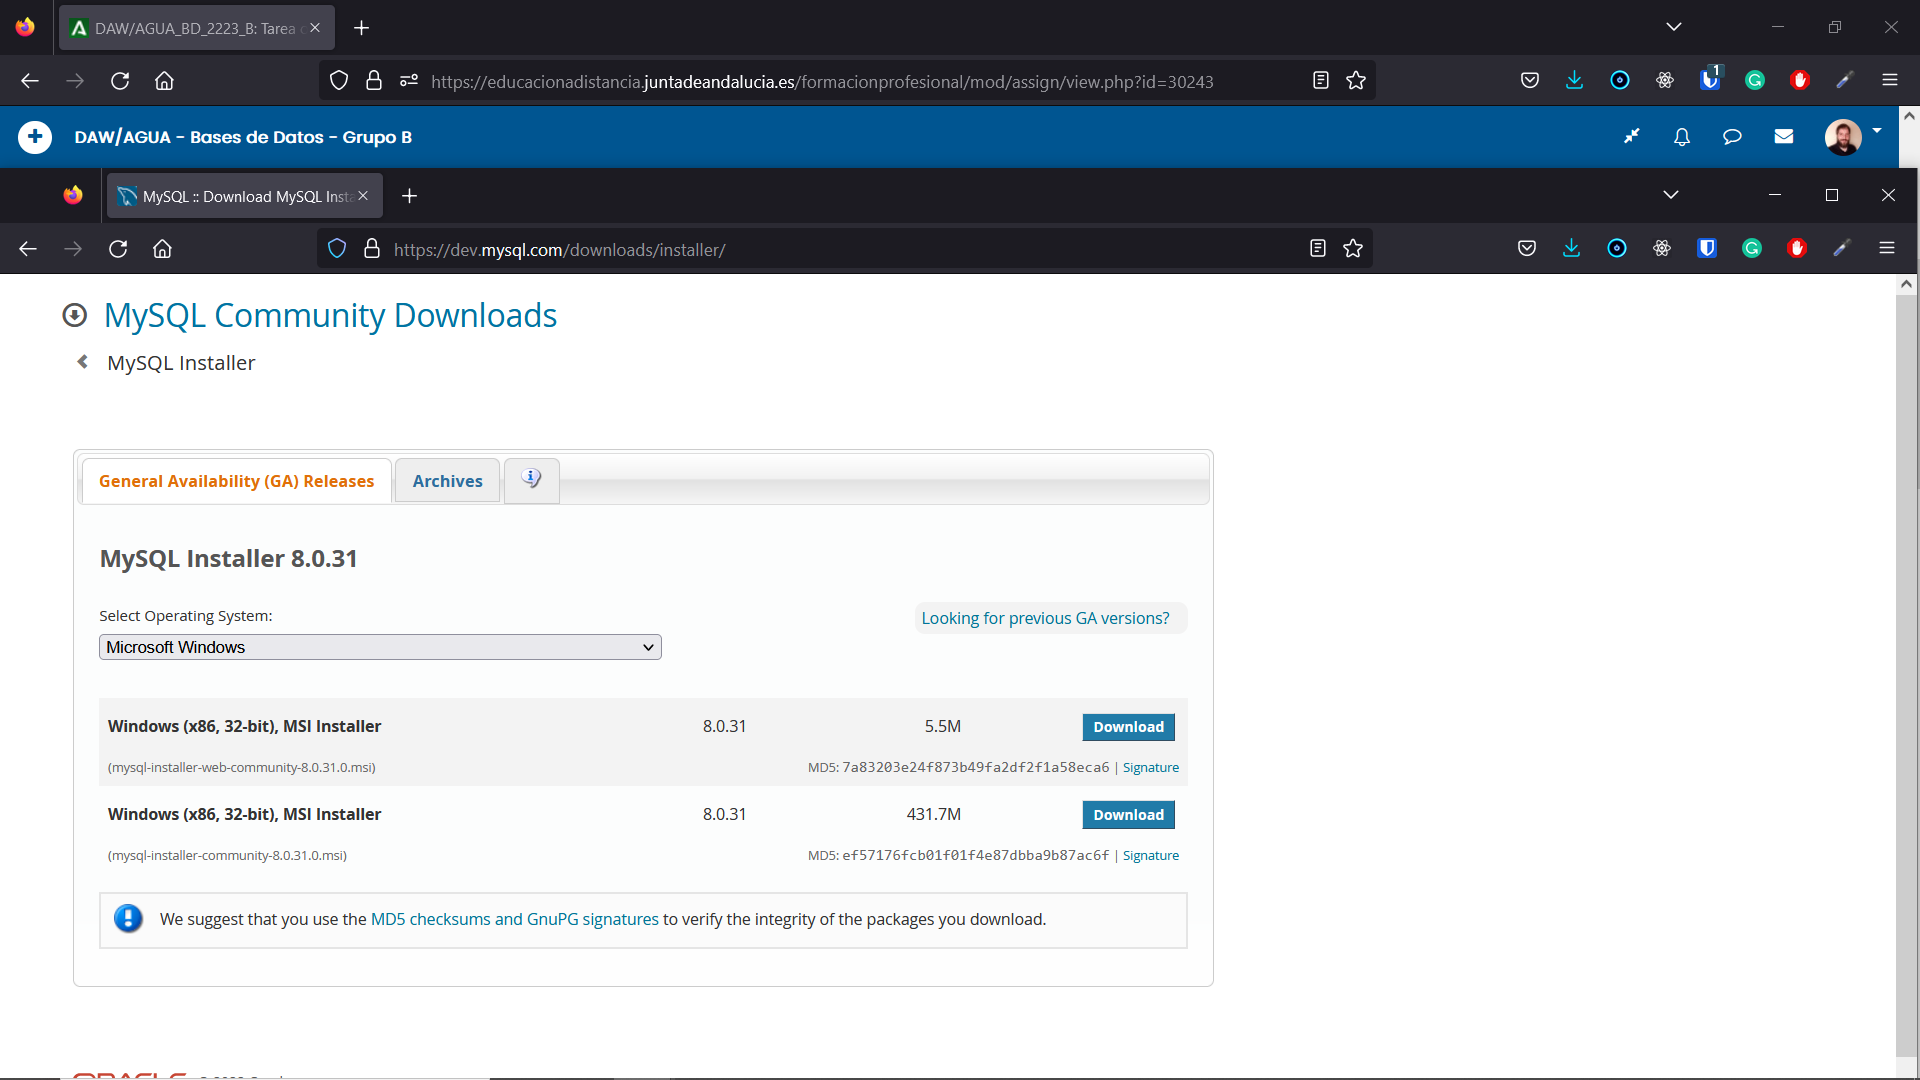
\includegraphics[scale=0.32]{descarga-mysql.png}
        \caption{Página de descarga del instalador de MySQL}
    \end{figure}

    \item \textbf{Instalación}

    Una vez descargado el instalador, lo ejecutamos desde el directorio donde se haya descargado. Esto iniciará el instalador, mostrando una ventana donde nos permitirá elegir que versión de MySQL queremos instalar. Nosotros vamos a elegir la \textbf{Developer Default}, que nos instalará todas las herramientas necesarias para el desarrollo, como podemos ver en la siguiente figura. Una vez seleccionada la opción, pulsaremos en botón ``\textit{Next}''.

   \begin{figure}[ht]
        \centering
        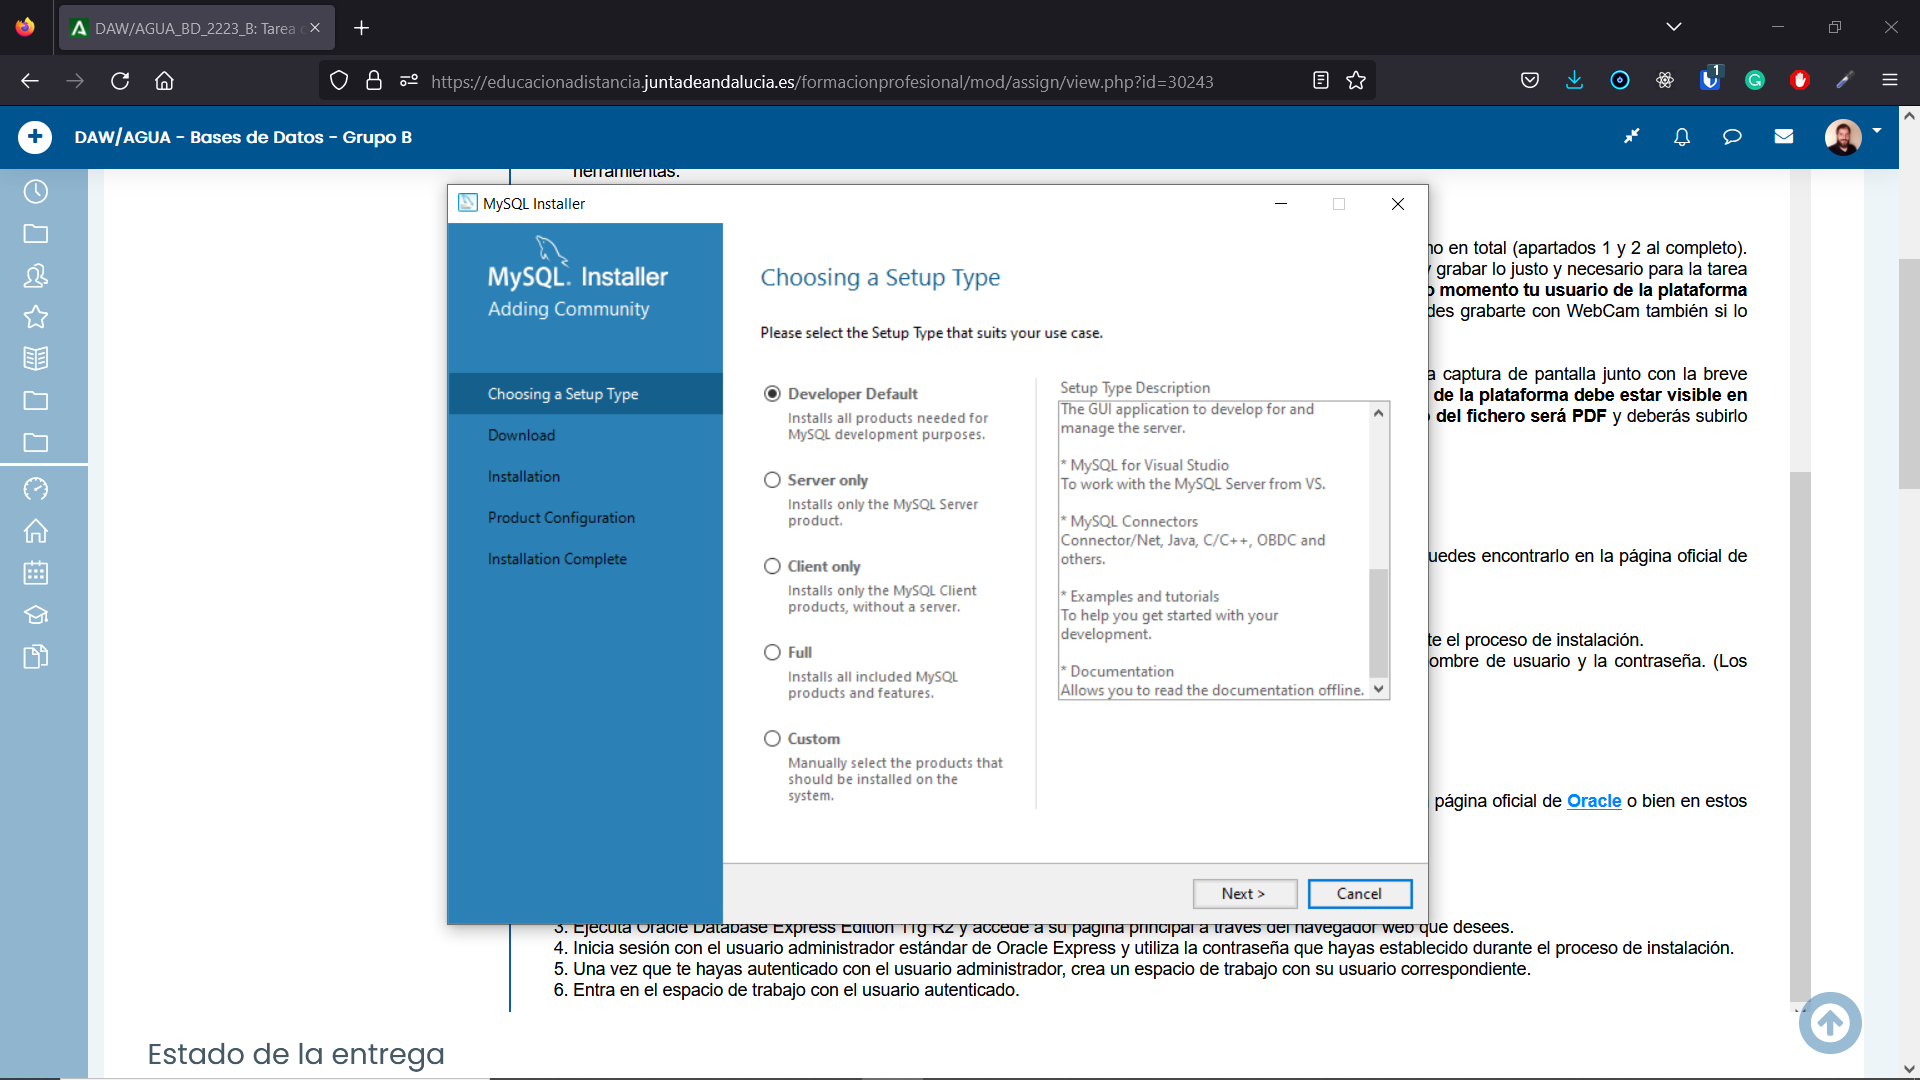
\includegraphics[scale=0.30]{install-mysql-1.png}
        \caption{Pantalla inicial del Instalador de MySQL}
    \end{figure}

    Se nos puede mostrar alguna ventana indicándonos que hay dependencias sin cumplir, por ejemplo, en el caso de que no tengamos instalado el editor Visual Studio. Podemos pulsar en ``\textit{Next}'' sin problema.

    A continuación se nos mostrará una pantalla con todos los componentes que se van a instalar. Pulsamos en ``\textit{Execute}'' y los componentes comenzarán a descargarse y a instalarse, como se puede observar en la siguiente figura.

    \begin{figure}[ht]
        \centering
        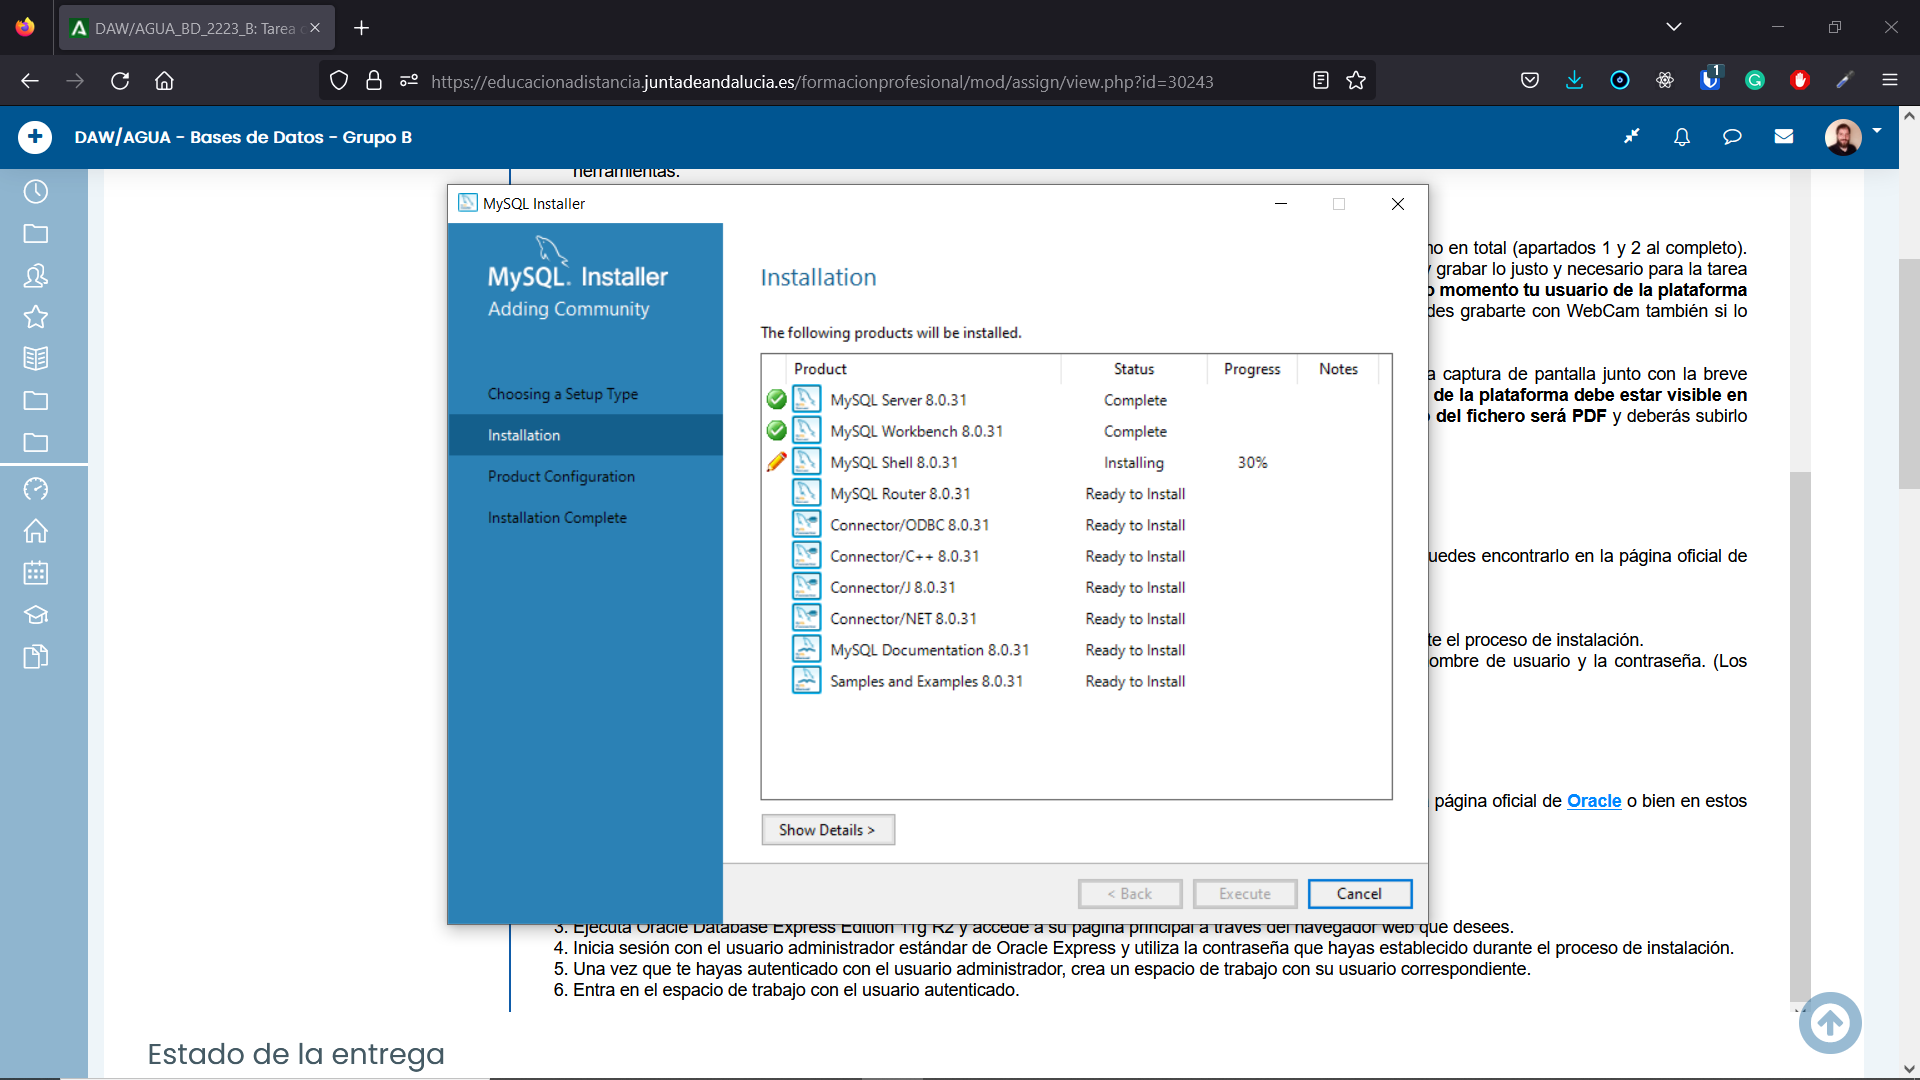
\includegraphics[scale=0.30]{install-mysql-2.png}
        \caption{Descarga e Instalación de componente de MySQL}
    \end{figure}

    Tras la descarga e instalación de componentes, se nos mostrarán diversas pantallas de configuración, aunque como nosotros vamos a seleccionar la configuración por defecto, solo deberemos introducir la \textbf{contraseña de root} en la pantalla que se nos solicite, dejando el resto de datos tal cuál y pulsando en el botón ``\textit{Next}'' hasta que se nos indique que la instalación se ha completado.

    \item \textbf{Ejecución de Workbench y Pantalla Principal}

    Después de realizar la instalación, buscaremos en el menú desplegable de Windows las aplicaciones instaladas. En concreto, vamos a ejecutar \textbf{MySQL Wokbench}, que es la interfaz gráfica oficial de MySQL. Pulsamos en esta aplicación y se nos abrirá la ventana principal. En esta pantalla principal podemos diferenciar los siguientes  elementos:

    \begin{enumerate}[label=\arabic*.]
        \item \textbf{Menu Principal}: contiene diferentes opciones como \textit{file}, \textit{edit}, \textit{view}, etc...
        \item \textbf{Menú Lateral}: donde podemos alternar entre diferentes vistas de la aplicación.
        \item \textbf{Enlaces}: diversos enlaces para acceder a la documentación, los foros o el blog.
        \item \textbf{MySQL Connections}: donde se nos mostrarán las diferentes conexiones que podemos realizar con la base de datos, donde podemos ver que solo tenemos la conexión por defecto creada con el usuario root
    \end{enumerate}

    En la siguiente captura, podemos ver todos estos elementos.

    \begin{figure}[ht]
        \centering
        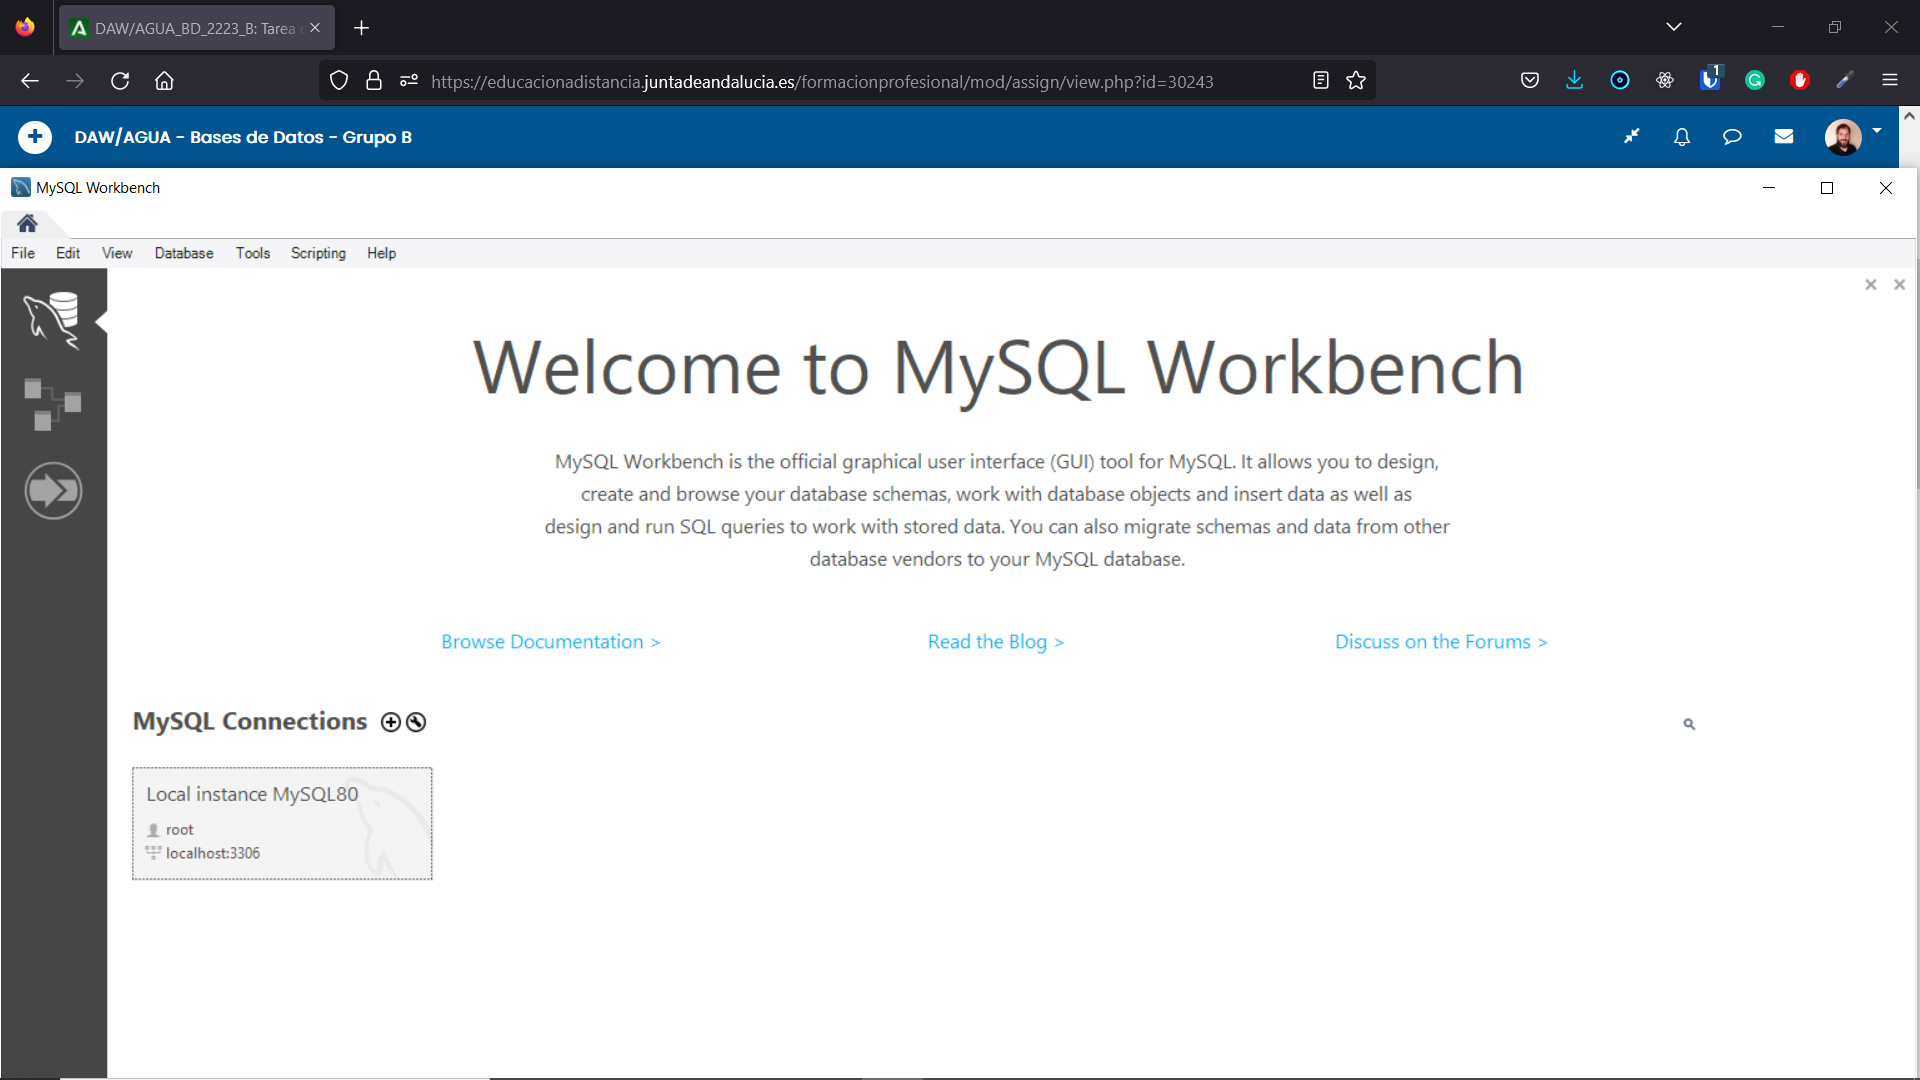
\includegraphics[scale=0.30]{workbench-main.png}
        \caption{Pantalla principal de MySQL Workbench}
    \end{figure}


    \item \textbf{Realizando la Primera Conexión}

    El siguiente paso es realizar una conexión con la base de datos. Ahora mismo solo tenemos la conexión creada durante la instalación para el \textbf{usuario root}, como hemos indicado en el punto anterior. Pulsamos sobre dicha conexión en el apartado \textbf{MySQL Connections} de la pantalla principal y se nos abrirá una ventana pidiéndonos la \textbf{contraseña del usuario root}, que deberíamos haber introducido durante el proceso de instalación.

    Después de haber introducido la contraseña, se realizará la conexión y se nos mostrará la página principal de la conexión, donde se nos permitirá gestionar la base de datos, realizar consultar, etc... Esta pantalla, esta compuesta de los siguientes elementos:

    \begin{enumerate}[label=\arabic*.]
        \item \textbf{Menu Principal y Barra de Herramientas}: en la parte superior nos encontramos el menú principal, con diferentes opciones y desplegables y la barra de herramientas, que nos permite realizar acciones rápidamente, como añadir tablas a la base de datos, filas a una tabla, columnas, etc...
        \item \textbf{Menu Lateral}: este menú nos permite administrar diferentes aspectos de la base de datos, como las conexiones que se han realizado, el número de usuario y sus privilegios, el estado del sistema, etc.., así como consultar diferente información sobre la base de datos como los logs, la performance, etc...
        \item \textbf{Pestaña de Consultas}: en esta pestaña es donde realizare las consultas a la base de datos, usando para ello, principalmente, el lenguaje SQL.
        \item \textbf{Pestaña SQL Additions}: esta pestaña nos permite cargar diferentes herramientas que nos ayudarán a la hora de realizar las consultas, como por ejemplo, snippets para SQL.
        \item \textbf{Pestaña de Salida}: aquí se nos mostrará la salida de las acciones realizadas.
    \end{enumerate}

    \begin{figure}[ht]
        \centering
        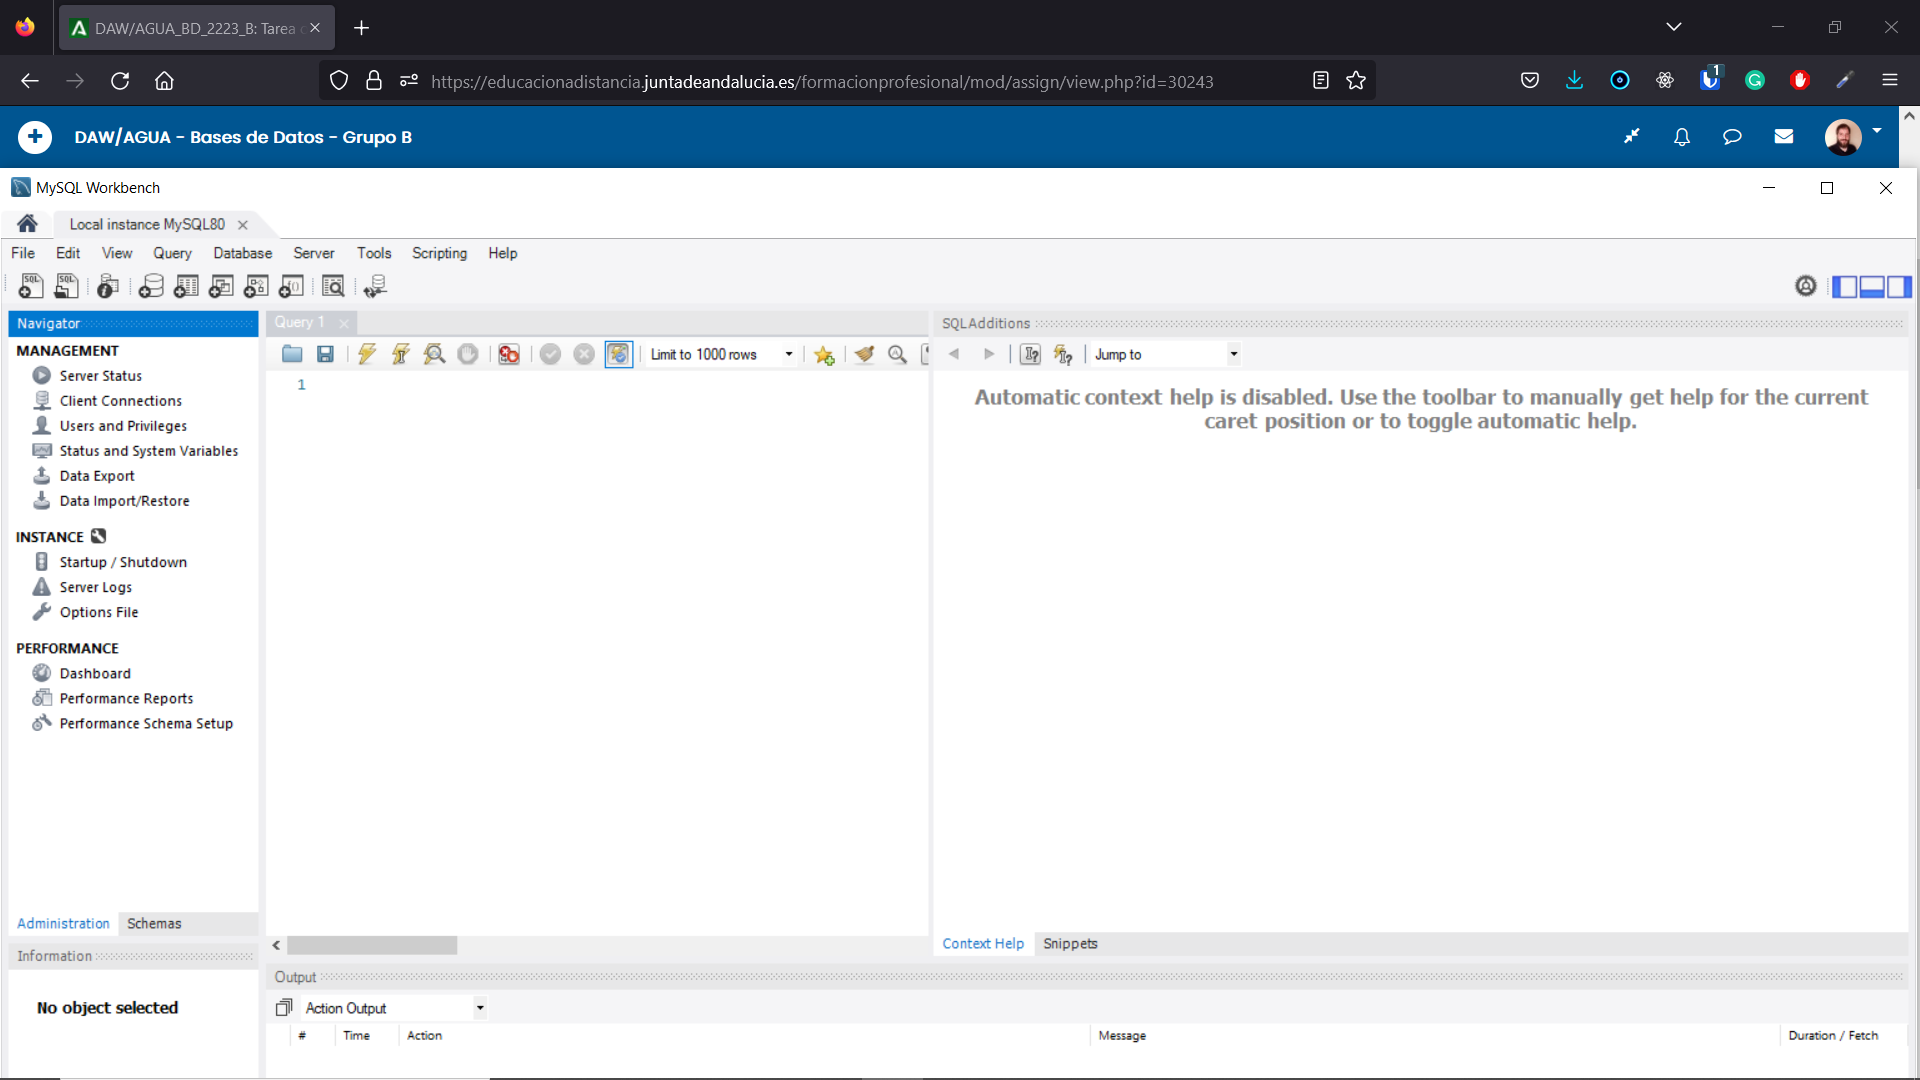
\includegraphics[scale=0.30]{workbench-conection-2.png}
        \caption{Ventana emergente para realizar la conexión con la base de datos}
    \end{figure}

    \item \textbf{Creación de Usuario}

    Ya que tenemos una nueva conexión activa y con privilegios de administrador vamos a crear una nuevo usuario. Para ello, pulsamos en el opción ``\textit{Users and Privileges}'' del menú lateral en la ventana principal de conexión. Estos nos abrirá una nueva ventana donde se nos mostrará los usuarios que hay ahora mismo creados en la base de datos.

    Pulsamos en la opción ``\textit{Add Account}'', que nos encontramos abajo a la izquierda, y se nos abrirá un formulario donde podremos introducir diferentes datos sobre el nuevo usuario. En nuestro caso, solo vamos a cambiar el \textbf{nombre de usuario} a y a introducir \textbf{una contraseña}. Debemos introducir una contraseña que nos sea fácil de recordar, aunque hay que tener en cuenta en en entornos de producción esto sería un error muy grande, ya que las contraseña tienen que ser suficientemente fuertes y complejas para no comprometer la seguridad de la base de datos.

    Una vez que hayamos introducido la información, pulsamos en el botón ``\textit{Apply}'' y nuestro usuario se habrá creado. En la siguiente figura podemos ver una captura de la pestaña de creación de usuarios.

    \newpage

    \begin{figure}[ht]
        \centering
        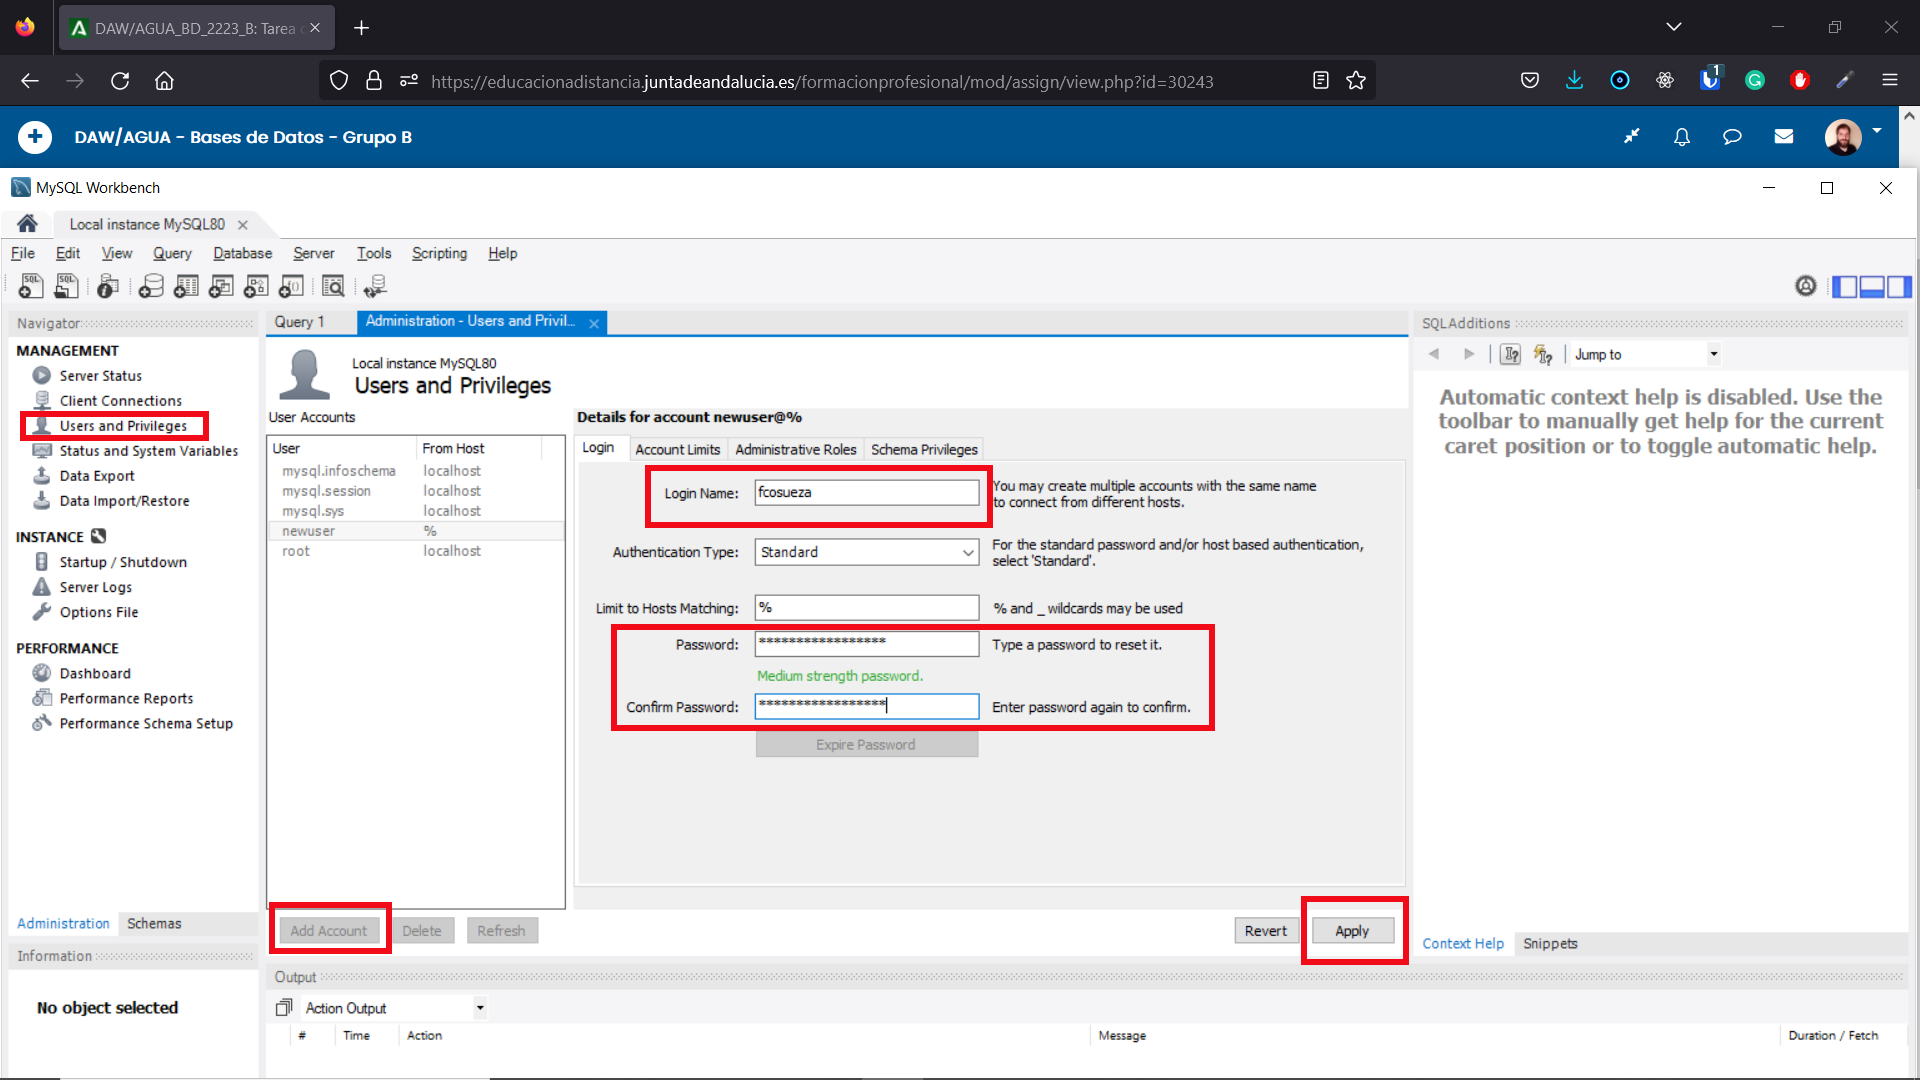
\includegraphics[scale=0.30]{create-user.png}
        \caption{Sección de Empleo Público del IAAP}
        \label{fig:create}
    \end{figure}

    \item \textbf{Conexión con el Nuevo Usuario}

    Una vez creado el usuario, ya solo nos queda realizar una conexión a la base de datos con éste.

    Primero cerramos la ventana de conexión abierta y volvemos al menú principal de Workbench. En esta pantalla, pulsamos el botón ``\textit{+}'' que nos encontramos en la sección \textbf{MySQL Connections}, lo que nos abrirá un formulario para la creación de una nueva conexión.

    En esta nueva ventana, solo vamos a cambiar el usuario, que deberemos introducir el que hemos creado en el paso anterior. El resto de datos, los dejaremos como están. En la siguiente captura, podemos ver el formulario de creación de una nueva conexión.

   \begin{figure}[ht]
        \centering
        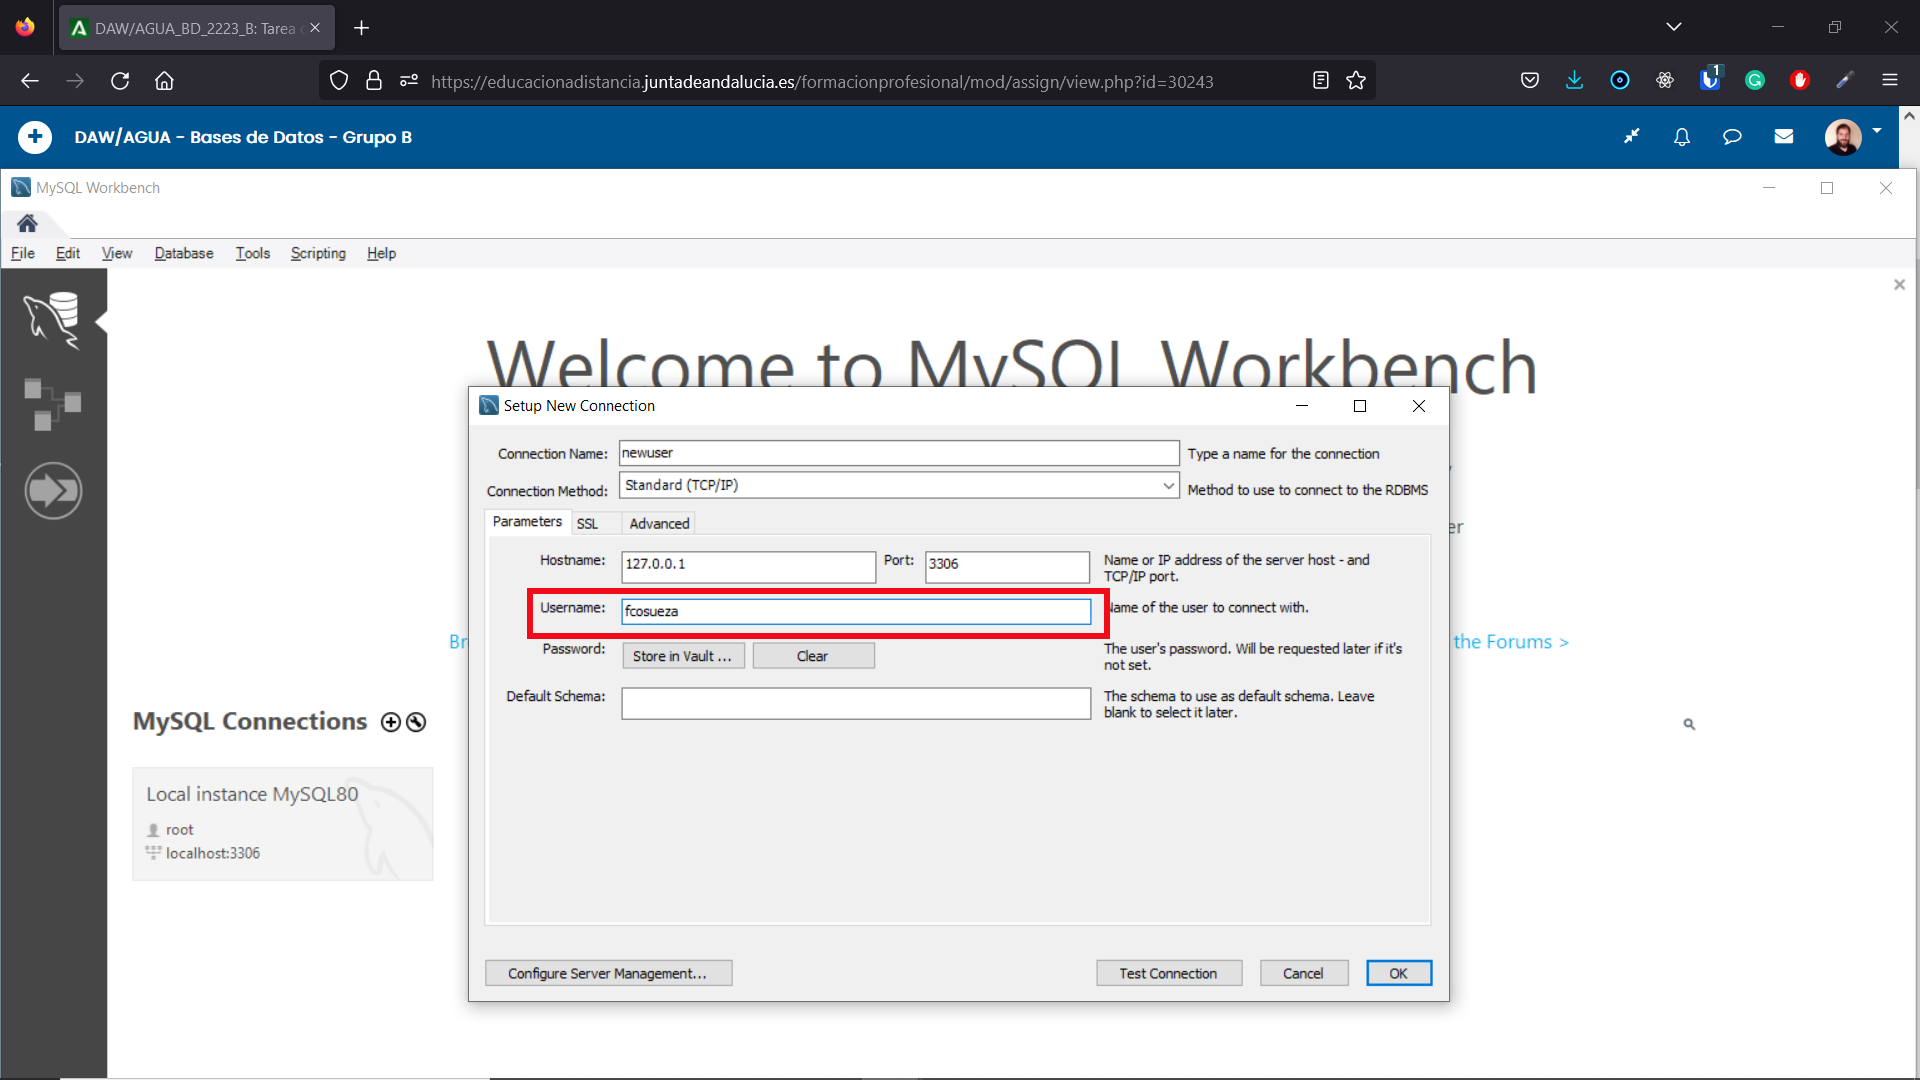
\includegraphics[scale=0.30]{newuser-conection.png}
        \caption{Creación de una nueva conexión con la base de datos}
    \end{figure}

    Una vez introducido el nuevo usuario, si queremos, podemos comprobar que la nueva conexión es correcta, pulsando el botón ``\textit{Test Connection}''. Después pulsaremos el botón ``\textit{Ok}'' y la conexión con el nuevo usuario se habrá creado con éxito.
\end{enumerate}

\section{Instalación de OracleDB}
Oracle Database es un sistema de gestión de base de datos de tipo objeto-relacional (ORDBMS, por el acrónimo en inglés de Object-Relational Data Base Management System), desarrollado por Oracle Corporation, la empresa estadounidense de hardware y software. Este tipo de sistema mejora la gestión de grandes bases de datos y también aumenta el nivel de seguridad. Se basa en un esquema estructurado que solo está disponible para administradores autorizados. \cite{oracle}

En estas sección, vamos a realizar la instalación de la versión \textbf{Oracle Database Express 11g 2} en Windows 10. Para llevar a cabo la instalación, debemos seguir los siguientes pasos:

\begin{enumerate}
    \item \textbf{Descarga del Instalador}

    Lo primero que debemos hacer es descargarnos el instalador del SGBD. En la página oficial de Oracle las versiones antiguas, en concreto la 11g, está bastante escondido y es difícil llegar a los enlaces de descarga, por lo que nosotros lo vamos de descargar desde \href{https://www.filehorse.com/es/descargar-oracle-database-express/}{este enlace en Filehorse}. Nosotros vamos a descargar la versión de 64bits. En la siguiente captura, vemos la página de descarga.

    \begin{figure}[ht]
        \centering
        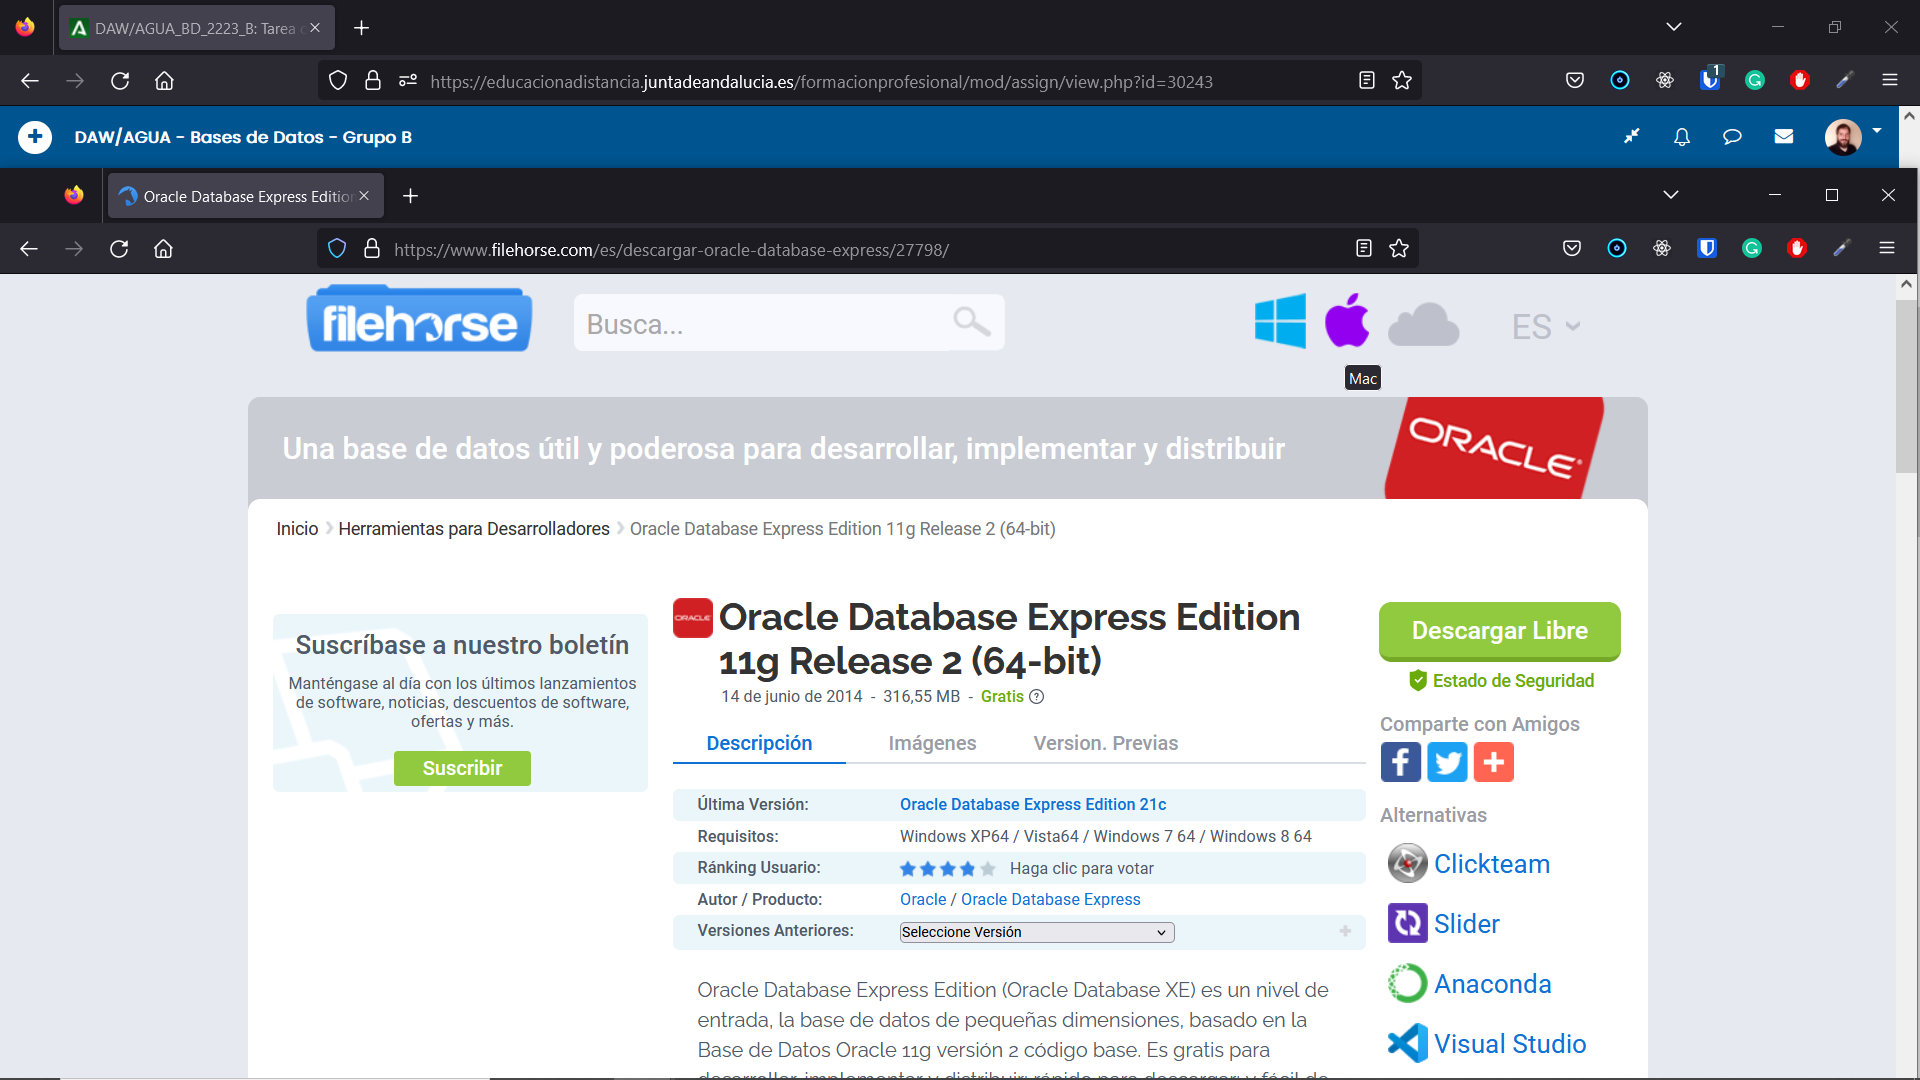
\includegraphics[scale=0.30]{download-oracle.png}
        \caption{Página de Filehorse para la descarga del instalador}
    \end{figure}

    Pulsando en el botón ``\textit{Descarga Libre}'' pasaremos a una página de confirmación y podemos comenzar la descarga.

    \item \textbf{Instalación}

    Una vez que hemos descargado el archivo, abriremos la carpeta donde se ha almacenado. El archivo descargado es un archivo comprimido por lo que deberemos descomprimirlo para realizar la instalación correctamente.

    Cuando hayamos descomprimido el archivo, entraremos en la carpeta \textbf{DISK1} creada buscaremos el archivo \textbf{setup}. Ejecutamos este archivo y el instalador se iniciará. Como podemos ver en la siguiente captura, el instalador nos dará la opción de seleccionar la versión de OracleDB que queremos instalar, en caso de que hubiera varias, nosotros vamos a seleccionar la única que hay, \textbf{Oracle Database 11g Express Edition}.

    \newpage

    \begin{figure}[ht]
        \centering
        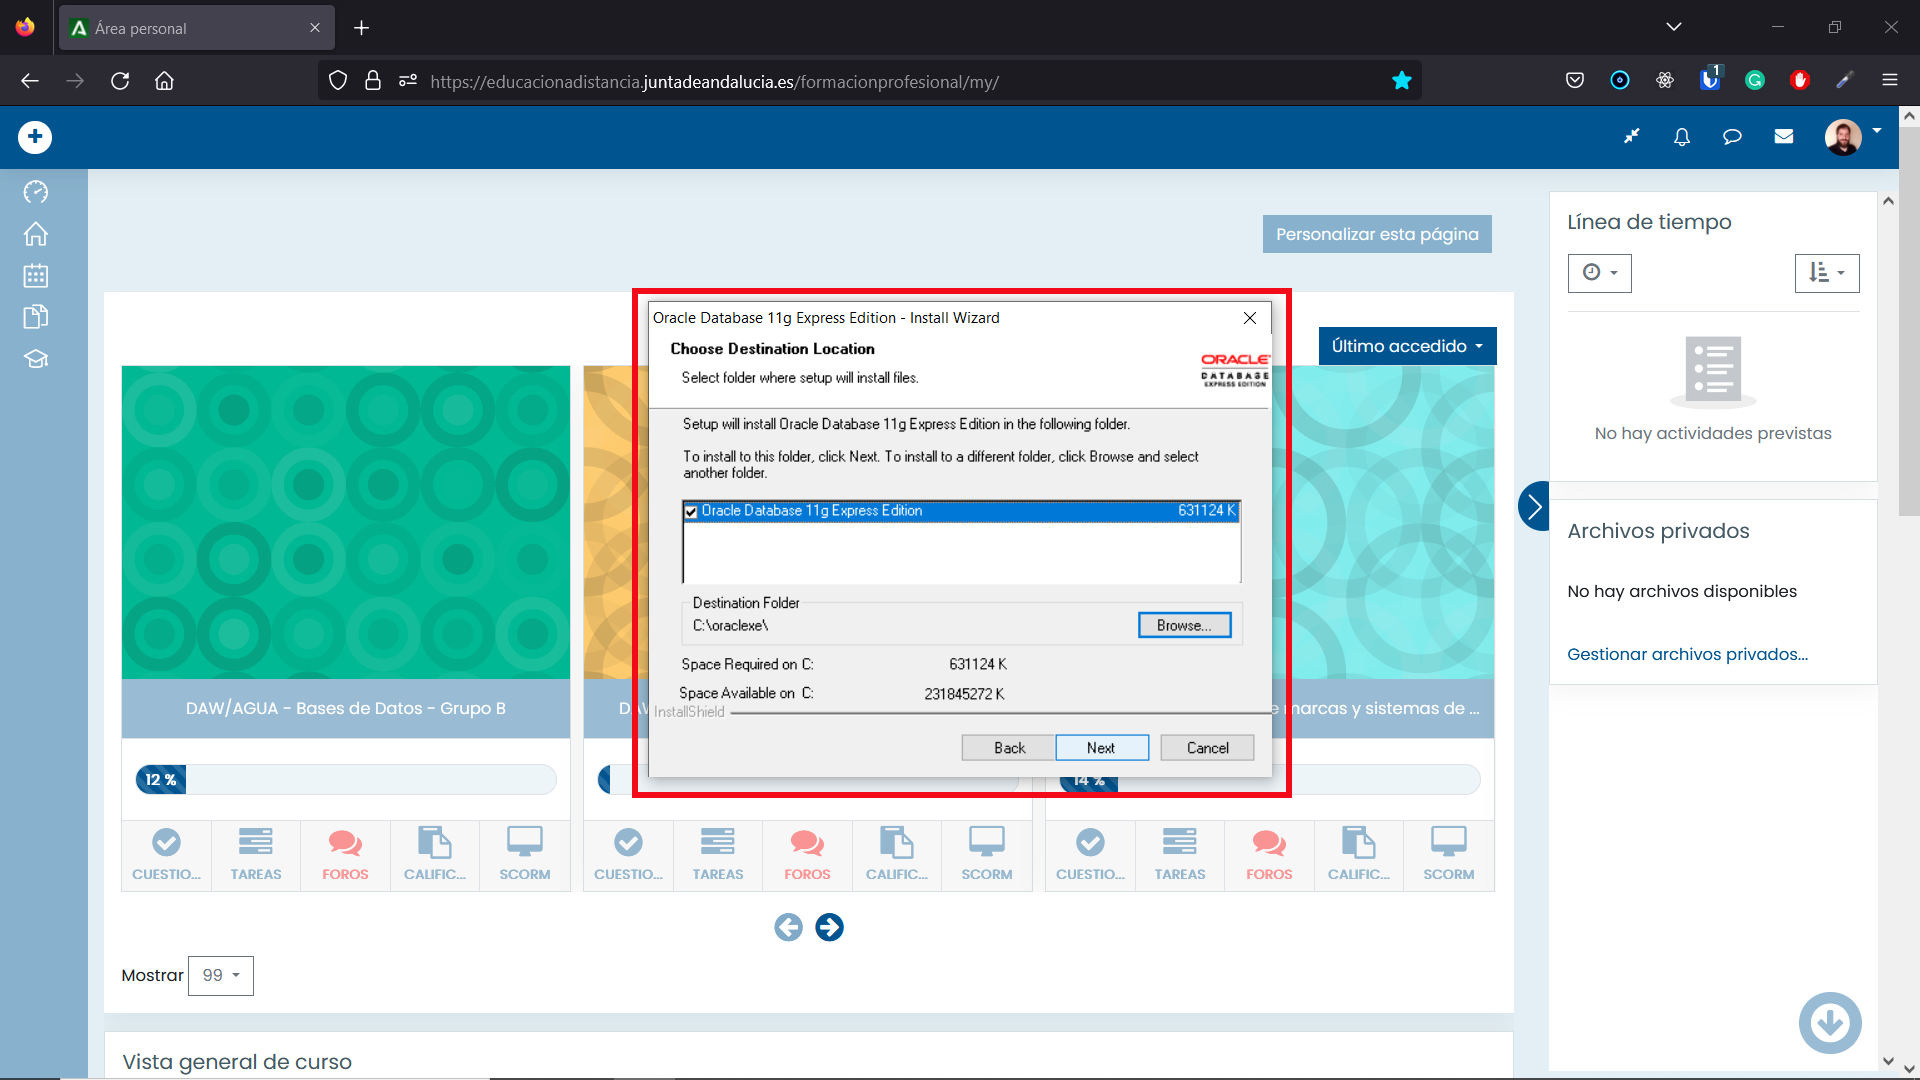
\includegraphics[scale=0.30]{install-oracle-1.png}
        \caption{Instalador de Oracle Database}
    \end{figure}

    Una vez que hayamos seleccionado la versión, comenzará la instalación. Durante el proceso, se nos pedirá que introduzcamos una contraseña. Esta contraseña será la empleada por los usuarios por defecto, SYS y SYSTEM, de OracleDB, así que debemos de recordarla. En la siguiente captura se muestra la confirmación de la nueva contraseña.

    \begin{figure}[ht]
        \centering
        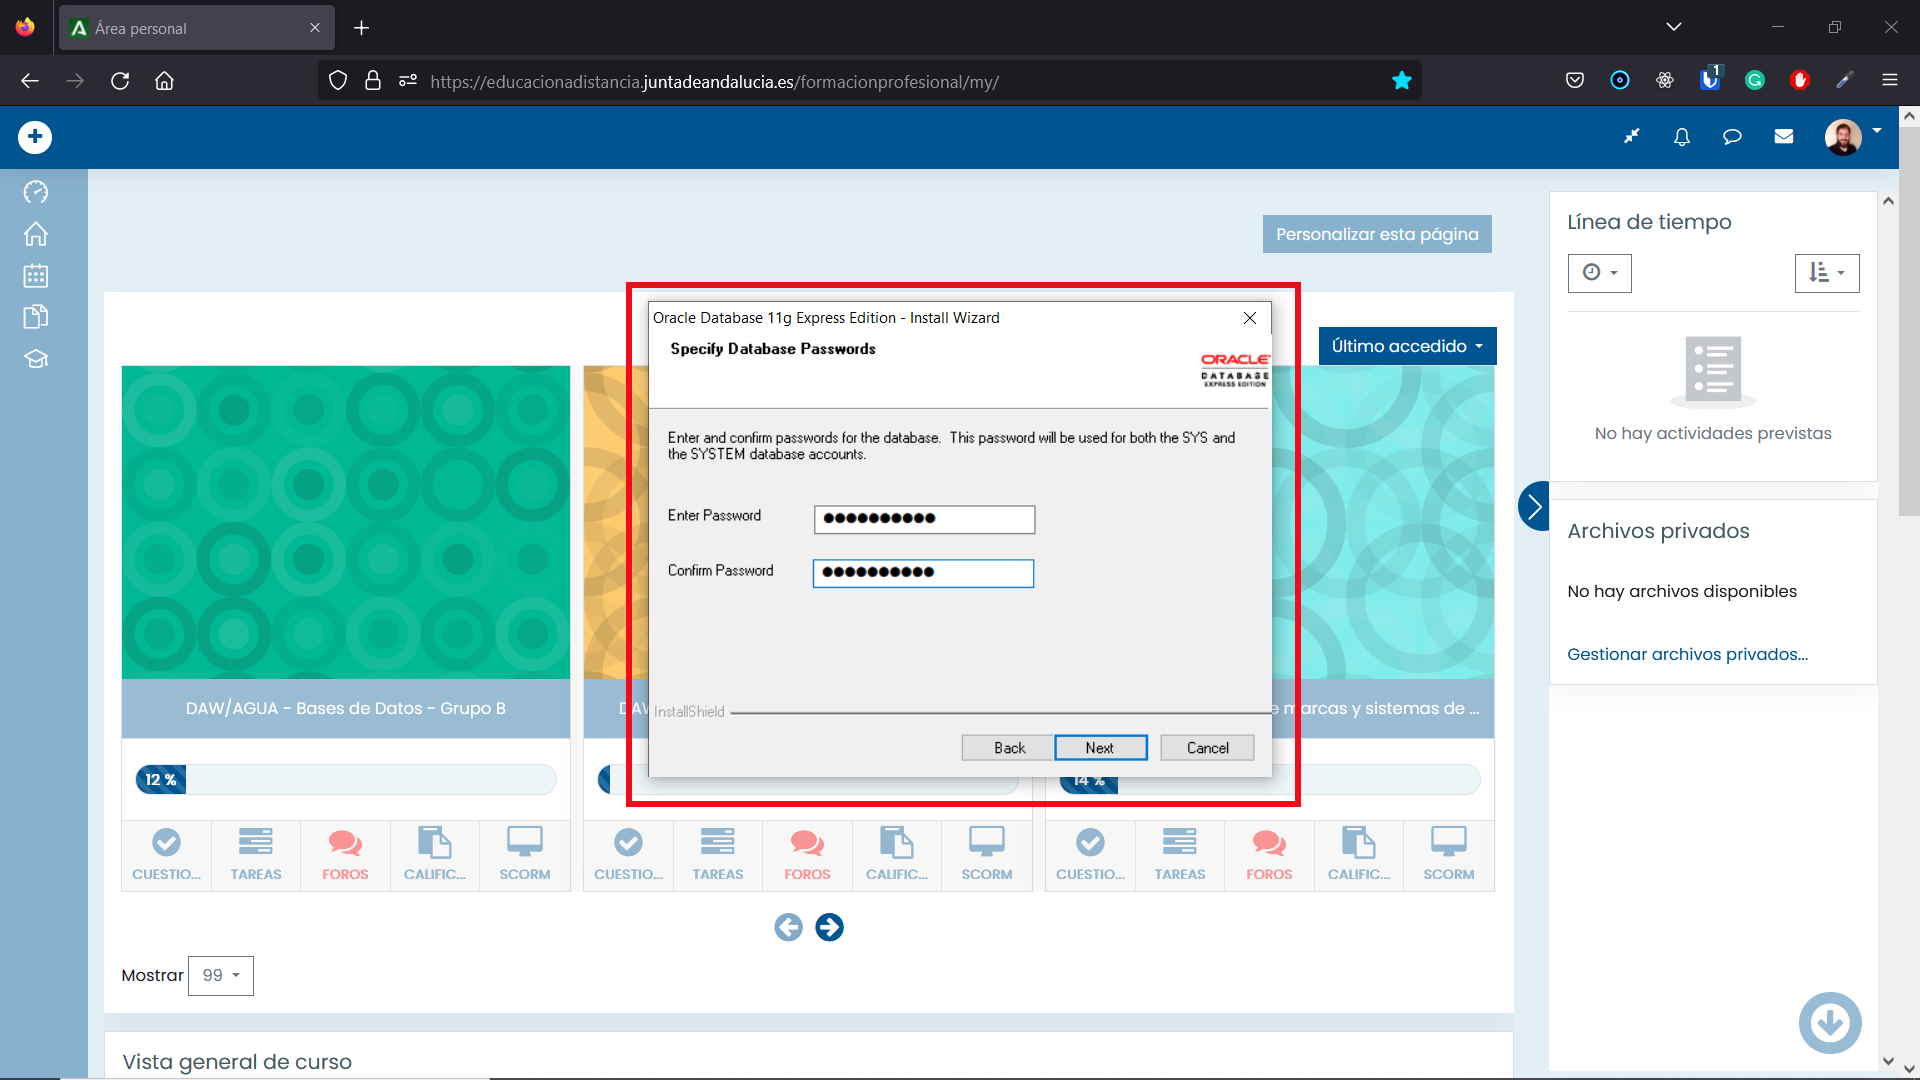
\includegraphics[scale=0.30]{install-oracle-2.png}
        \caption{Introducción de contraseña durante el proceso de instalación}
    \end{figure}

    Una vez que hayamos introducido la contraseña el proceso de instalación continuará con normalidad y nuestra base de datos quedará correctamente instalada.

    \item \textbf{Inicialización de OracleDB}

    Una vez realiza la instalación, se habrá creado e inicializado automáticamente una base de datos, ahora debemos acceder a ella para poder gestionarla.

    Si miramos en el escritorio de Windows, veremos que se ha creado un acceso directo llamado \textbf{Get Started with Oracle}, para acceder mediante la interface web, pulsamos este icono. Hay que tener en cuenta que pueden suceder dos cosas:

    \begin{itemize}
        \item \textbf{Ejecución Normal}: tras pulsar el icono se ejecutara correctamente y nos mostrará la pantalla inicial de OracleDB.
        \item \textbf{Error}: puede que al ejecutar el icono nos de un error del tipo ''\textit{No se puede encontrar el fichero ..."}, esto es debido a que la variable de entorno \textbf{HTTPPORT} no esta establecida, por lo que deberemos crear esa variable y asignarle el valor \textbf{8080}, tras lo que reiniciaremos el sistema. En este documento no se va a cubrir como crear variables de entorno en Windows, pero en \href{https://medium.com/@01luisrene/como-agregar-variables-de-entorno-s-o-windows-10-e7f38851f11f}{este articulo} hay un tutorial que puede ser de utilidad.

        Otra opción es copiar la dirección que se nos muestra en el mensaje de error, sustituir \textbf{HTTPPORT} por \textbf{8080} y copiarla en una navegador, aunque esta solución es mas engorrosa y deberemos realizar el procedimiento cada que que queramos conectar a la base de datos. Por lo que yo recomiendo crear la variables de entorno.
    \end{itemize}

    Cuando se haya ejecutado correctamente el acceso directo nos abrirá el navegador por defecto y nos mostrará la página principal de gestión de OracleDB, como podemos ver en la siguiente captura.

    \begin{figure}[ht]
        \centering
        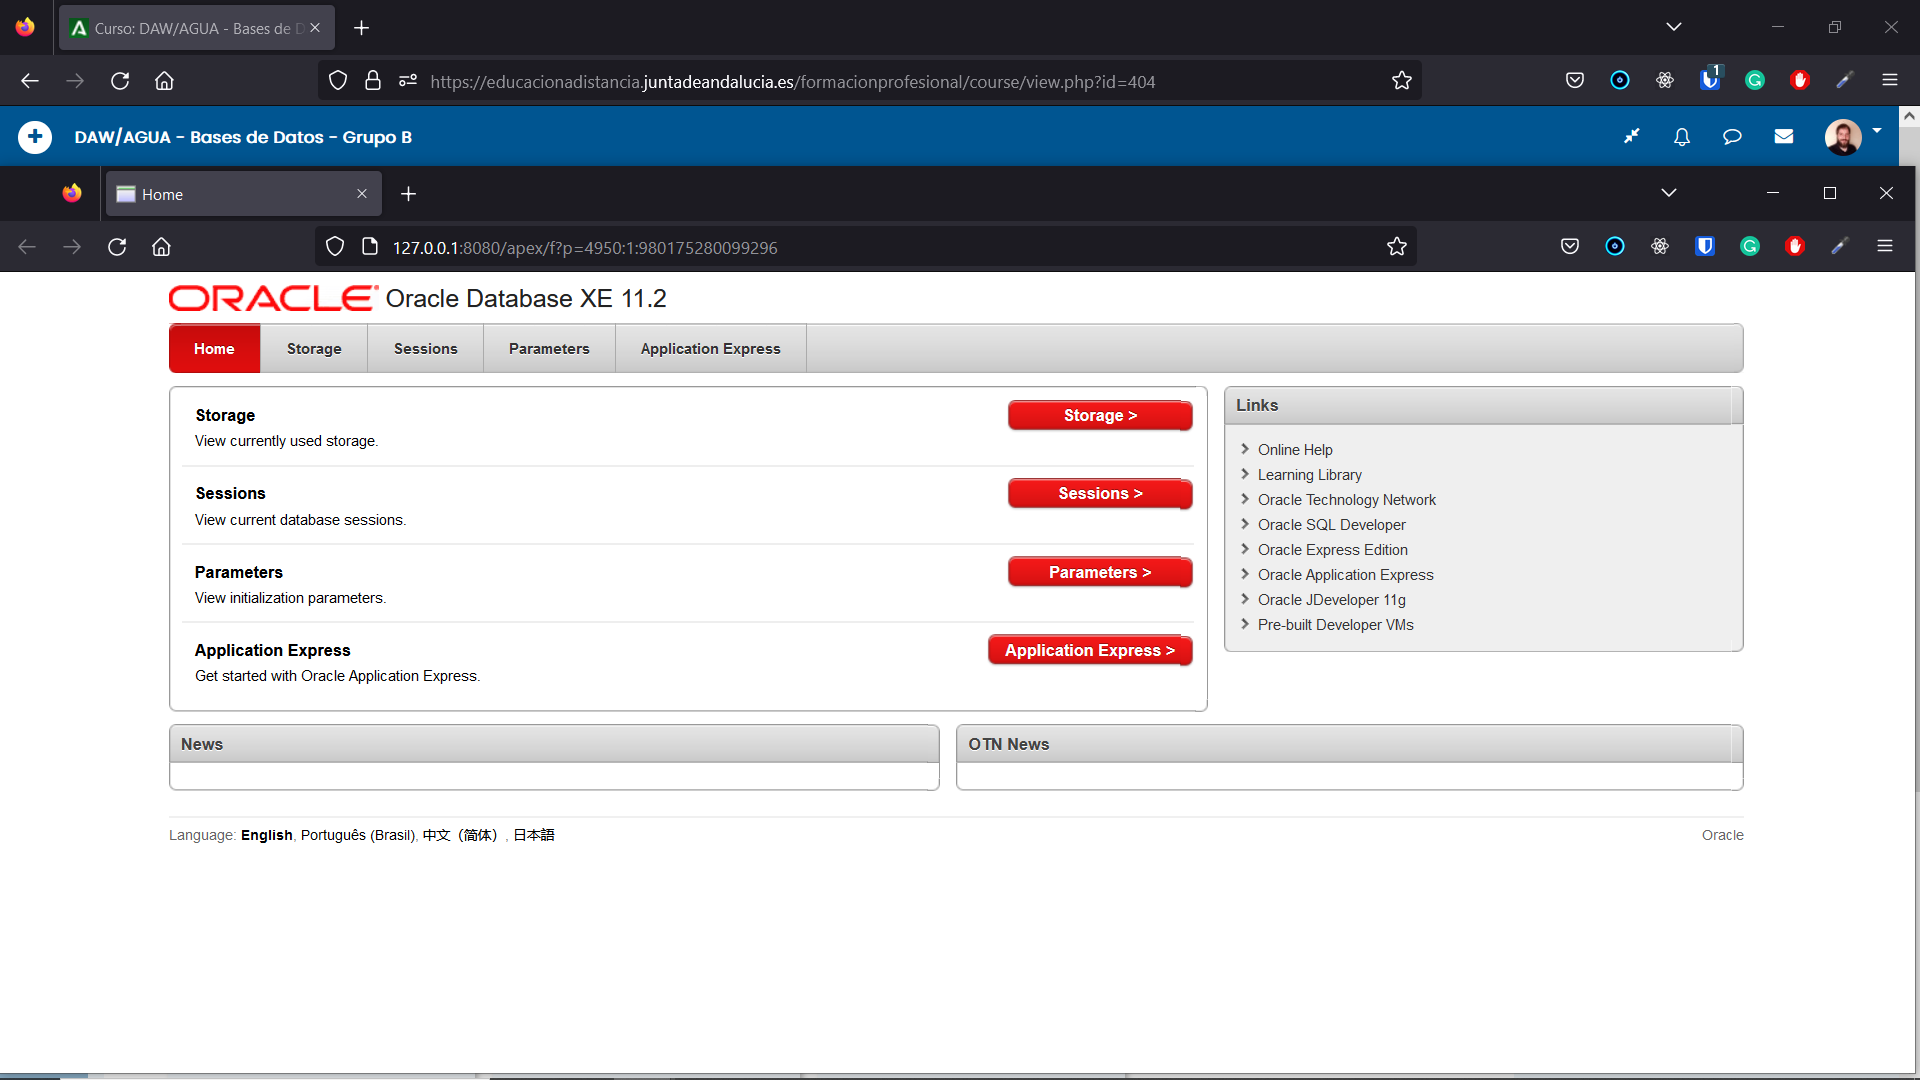
\includegraphics[scale=0.30]{oracle-main.png}
        \caption{Interfaz web de OracleDB}
    \end{figure}

    Como vemos en la captura, en la página principal tenemos diferentes secciones a las que podemos acceder tanto desde la barra superior como desde los enlaces que hay debajo. A la izquierda, tenemos un menú lateral con diferentes enlaces hacia la documentación de OracleDB.

    \item \textbf{Inicio de Sesión como Administrador}

    Desde la página principal de Oracle que hemos visto en el punto anterior, pulsamos en cualquier de los enlaces del menú. Independientemente del que pulsemos se nos mostrará un formulario para hacer \textit{login}.

    Deberemos introducir el usuario por defecto que tiene OracleDb, \textbf{SYSTEM}, y como contraseña la que hayamos introducido durante el proceso de instalación. Nuestro usuario quedará autentificado y ya podremos gestionar diferentes aspectos de la base de datos, aunque en esta guía solo vamos a crear un nuevo espacio de trabajo con un usuario como veremos en el siguiente paso.

    En la siguiente imagen, se muestra una captura del formulario de login para autentificar el usuario por defecto.

    \begin{figure}[ht]
        \centering
        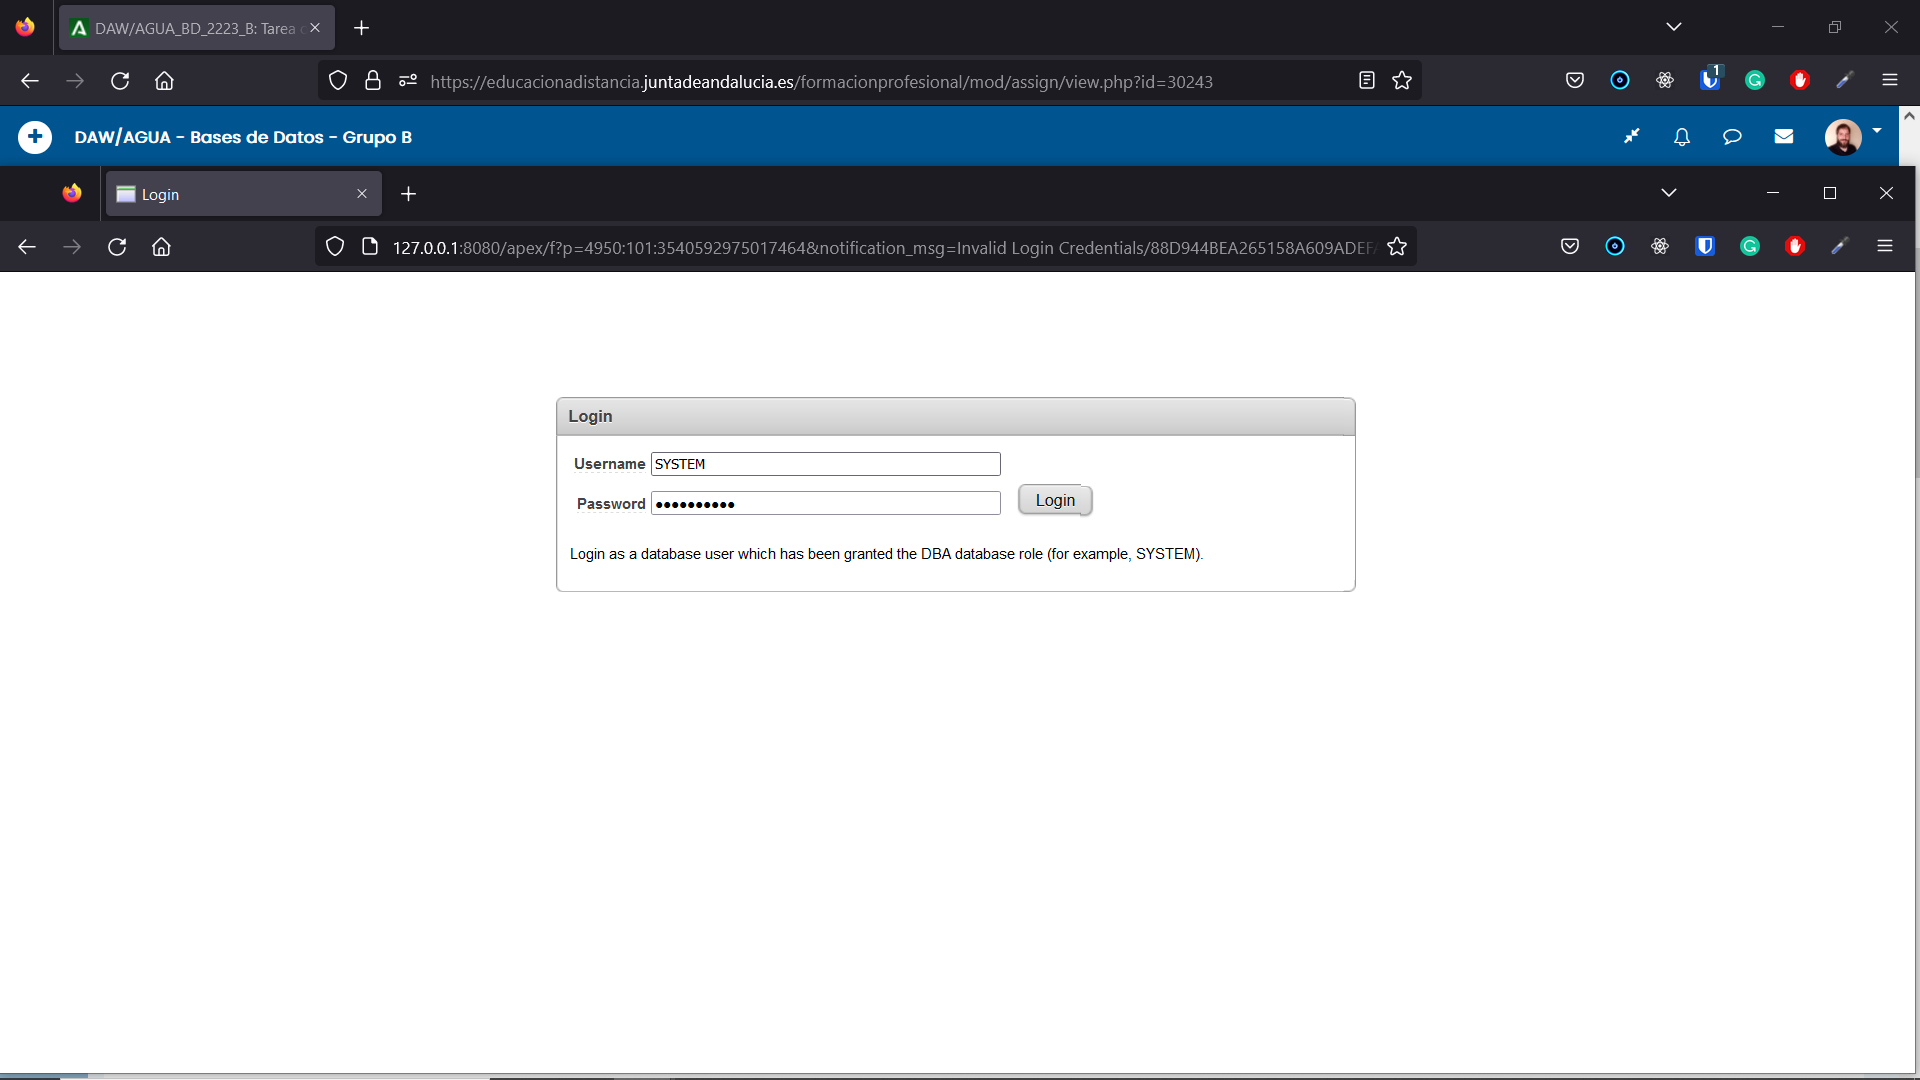
\includegraphics[scale=0.25]{oracle-login.png}
        \caption{Formulario de login inicial de OracleDB}
    \end{figure}

    \item \textbf{Creación de Espacio de Trabajo}

    Una vez que hayamos iniciado sesión, vamos a crear un nuevo espacio de trabajo con usuario asociado. Para ello, pulsamos en la opción ``\textit{Aplication Express}'' de la pantalla principal de Oracle, que nos llevará a la pantalla de creación. En esta pantalla tenemos dos secciones, una para crear un nuevo espacio de trabajo, la que vamos a usar ahora, y otra para iniciar sesión en un espacio de trabajo ya creado.

    Para crear el nuevo espacio de trabajo, introducimos el nombre del espacio de trabajo y el nombre de usuario, en nuestro caso hemos usado el mismo para para simplificarlo un poco. Una vez introducido, pulsamos en ``\textit{Create Workspace} y el espacio de trabajo se creará. En la siguiente captura, vemos una imagen de la pantalla de creación de espacios de trabajo.

    \begin{figure}[ht]
        \centering
        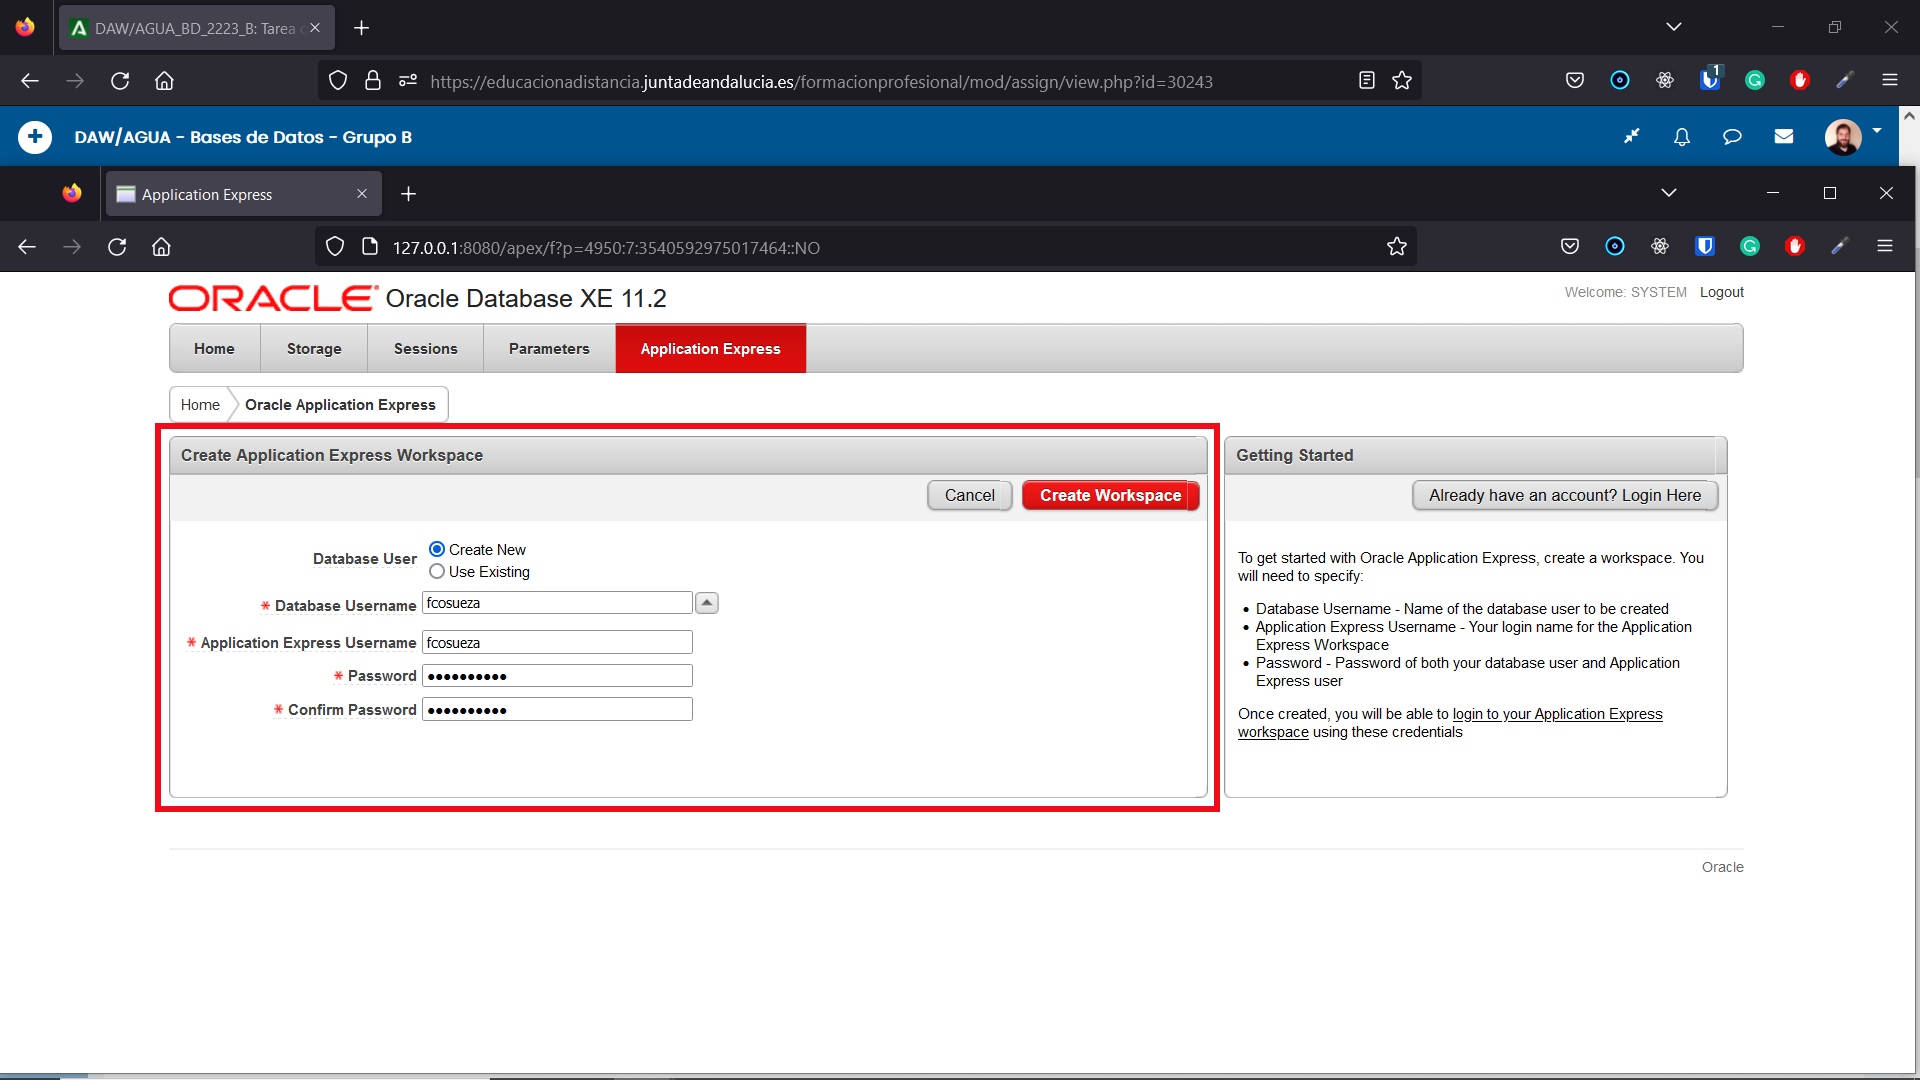
\includegraphics[scale=0.30]{oracle-newuser.png}
        \caption{Creación de usuario y espacio de trabajo en OracleDB}
    \end{figure}

    \item \textbf{Inicio de sesión en el Espacio de Trabajo Creado}

    Ya solo nos falta iniciar sesión con el nuevo usuario en el espacio de trabajo creado. Para ello, volvemos a la sección ``\textit{Aplication Express}'' del paso anterior, pero en vez de centrarnos en la sección para crear una espacio de trabajo, pulsamos en el botón ``\textit{Already have and account? Login Here}'' que se encuentra en la sección de la derecha ``\textit{Getting Started}''. Esto nos llevara a la pantalla de login de espacios de trabajo.

    Introducimos el nombre de usuario y del espacio de trabajo creados en está pantalla, así como la contraseña que hayamos puesto, como se ve en la siguiente captura.

     \begin{figure}[ht]
        \centering
        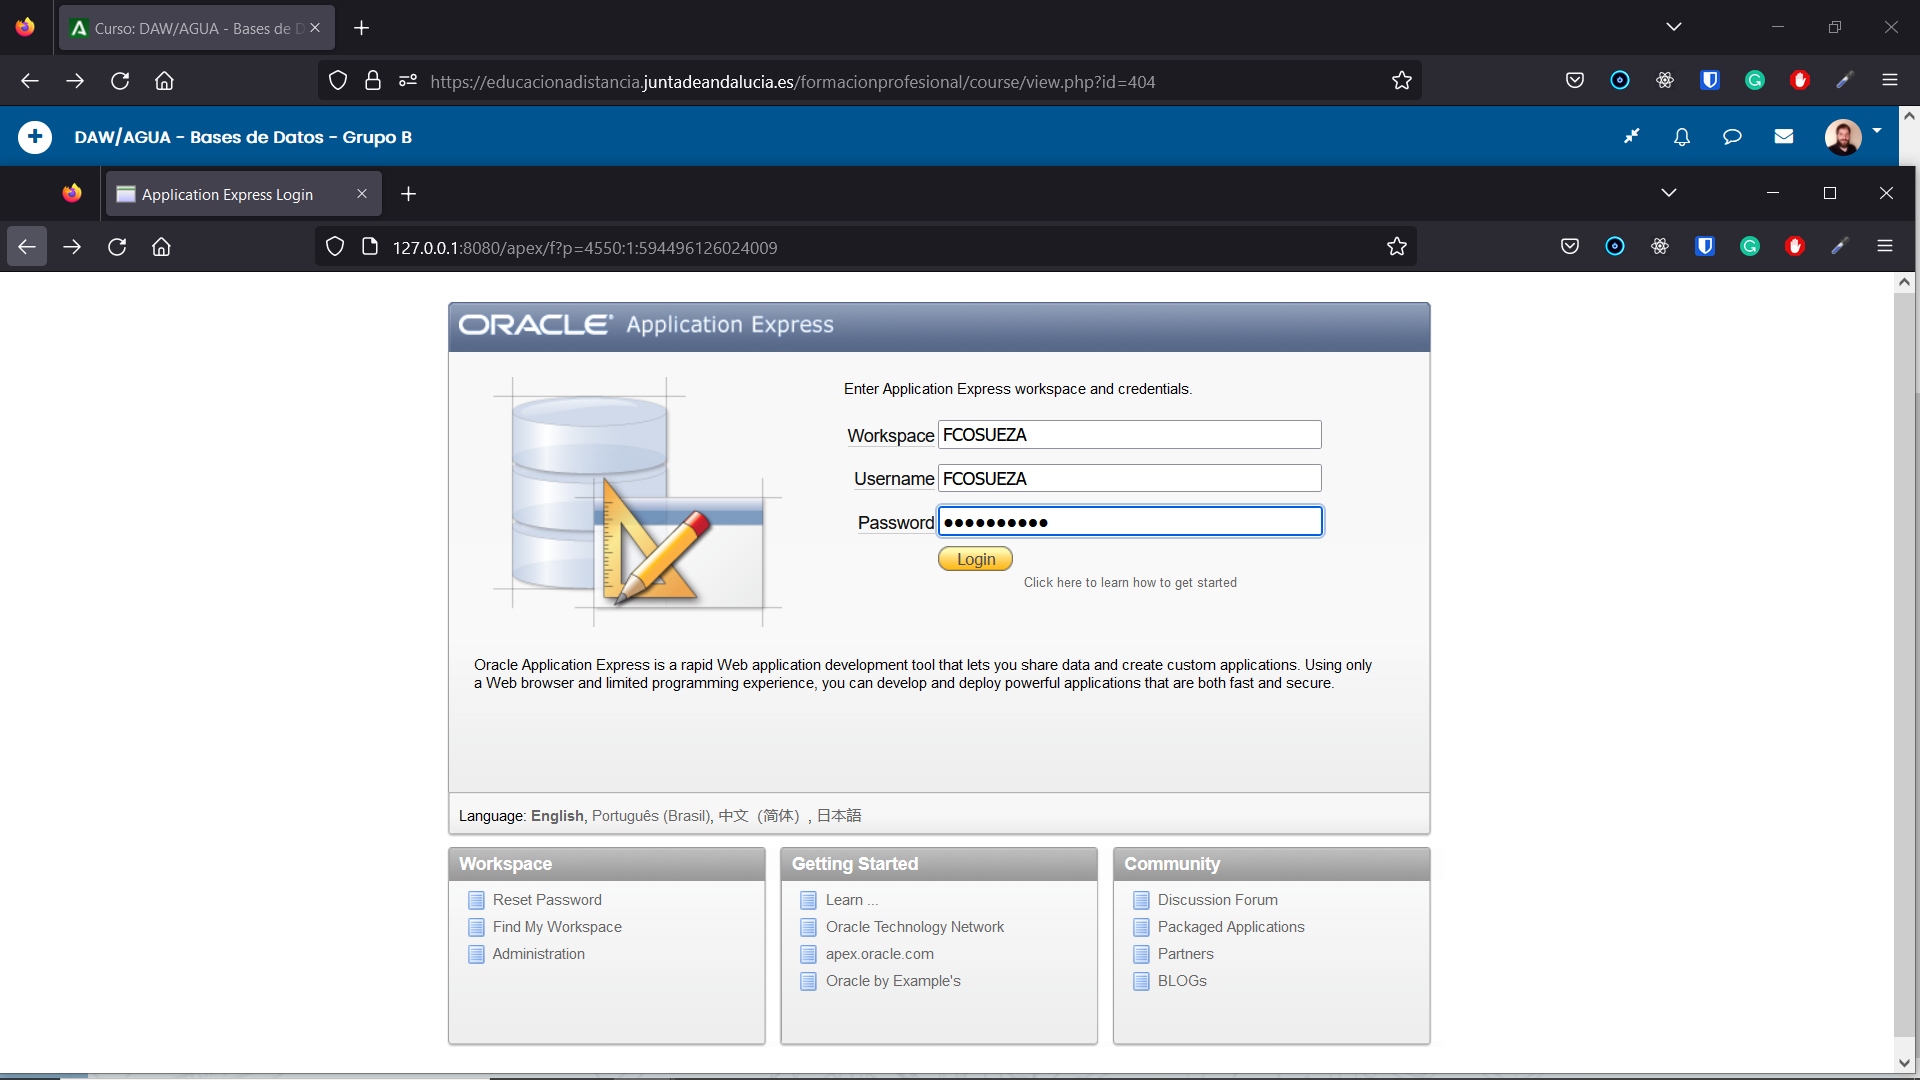
\includegraphics[scale=0.30]{login-new-user.png}
        \caption{Inicio de sesión con el nuevo usuario}
    \end{figure}

    Una vez introducido correctamente los datos, pulsamos en el botón ``\textit{Login}'' en iniciaremos sesión, abriéndose la página principal del espacio de trabajo, como vemos en la siguiente captura.

    \begin{figure}[ht]
        \centering
        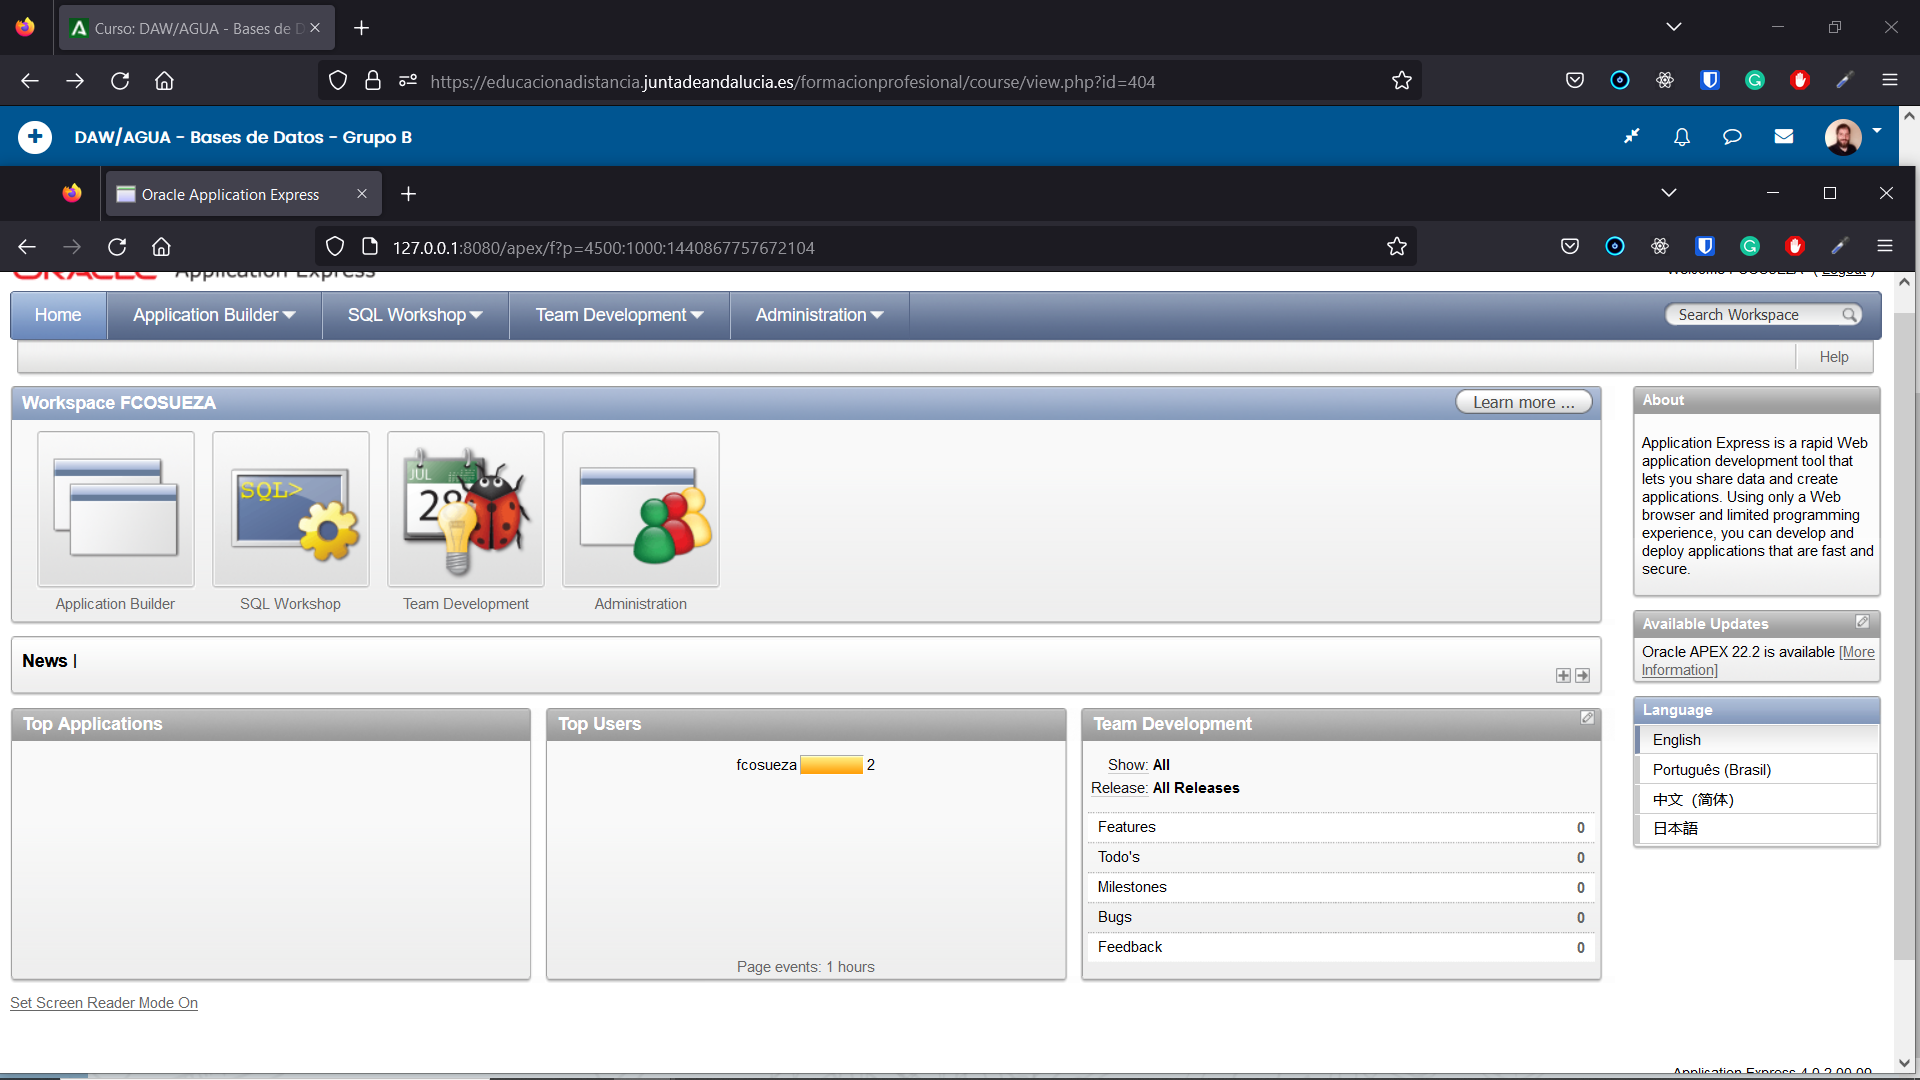
\includegraphics[scale=0.30]{newuser-workspace.png}
        \caption{Página principal del espacio de trabajo creado}
    \end{figure}
\end{enumerate}






% Bibliography

\newpage
\bibliography{citas}
\bibliographystyle{unsrt}

\end{document}